%Distance athlete’s æffect on urban rhythm How do ultrarunners run in automatized cities?


% ******************************* PhD Thesis Template **************************
% Please have a look at the README.md file for info on how to use the template

\documentclass[a4paper,12pt,times,numbered,print,index]{Classes/PhDThesisPSnPDF}

% ******************************************************************************
% ******************************* Class Options ********************************
% *********************** See README for more details **************************
% ******************************************************************************

% `a4paper'(The University of Cambridge PhD thesis guidelines recommends a page
% size a4 - default option) or `a5paper': A5 Paper size is also allowed as per
% the Cambridge University Engineering Deparment guidelines for PhD thesis
%
% `11pt' or `12pt'(default): Font Size 10pt is NOT recommended by the University
% guidelines
%
% `oneside' or `twoside'(default): Printing double side (twoside) or single
% side.
%
% `print': Use `print' for print version with appropriate margins and page
% layout. Leaving the options field blank will activate Online version.
%
% `index': For index at the end of the thesis
%
% `draftclassic': For draft mode without loading any images (same as draft in book)
%
% `draft': Special draft mode with line numbers, images, and water mark with
% timestamp and custom text. Position of the text can also be modified.
%
% `abstract': To generate only the title page and abstract page with
% dissertation title and name, to submit to the Student Registry
%
% `chapter`: This option enables only the specified chapter and it's references
%  Useful for review and corrections.
%
% ************************* Custom Page Margins ********************************
%
% `custommargin`: Use `custommargin' in options to activate custom page margins,
% which can be defined in the preamble.tex. Custom margin will override
% print/online margin setup.
%
% *********************** Choosing the Fonts in Class Options ******************
%
% `times' : Times font with math support. (The Cambridge University guidelines
% recommend using times)
%
% `fourier': Utopia Font with Fourier Math font (Font has to be installed)
%            It's a free font.
%
% `customfont': Use `customfont' option in the document class and load the
% package in the preamble.tex
%
% default or leave empty: `Latin Modern' font will be loaded.
%
% ********************** Choosing the Bibliography style ***********************
%
% `authoryear': For author-year citation eg., Krishna (2013)
%
% `numbered': (Default Option) For numbered and sorted citation e.g., [1,5,2]
%
% `custombib': Define your own bibliography style in the `preamble.tex' file.
%              `\RequirePackage[square, sort, numbers, authoryear]{natbib}'.
%              This can be also used to load biblatex instead of natbib
%              (See Preamble)
%
% **************************** Choosing the Page Style *************************
%
% `default (leave empty)': For Page Numbers in Header (Left Even, Right Odd) and
% Chapter Name in Header (Right Even) and Section Name (Left Odd). Blank Footer.
%
% `PageStyleI': Chapter Name next & Page Number on Even Side (Left Even).
% Section Name & Page Number in Header on Odd Side (Right Odd). Footer is empty.
%
% `PageStyleII': Chapter Name on Even Side (Left Even) in Header. Section Number
% and Section Name in Header on Odd Side (Right Odd). Page numbering in footer


% ********************************** Preamble **********************************
% Preamble: Contains packages and user-defined commands and settings
% ******************************************************************************
% ****************************** Custom Margin *********************************

% Add `custommargin' in the document class options to use this section
% Set {innerside margin / outerside margin / topmargin / bottom margin}  and
% other page dimensions
\ifsetCustomMargin
  \RequirePackage[left=37mm,right=30mm,top=35mm,bottom=30mm]{geometry}
  \setFancyHdr % To apply fancy header after geometry package is loaded
\fi

% Add spaces between paragraphs
%\setlength{\parskip}{0.5em}
% Ragged bottom avoids extra whitespaces between paragraphs
\raggedbottom
% To remove the excess top spacing for enumeration, list and description
%\usepackage{enumitem}
%\setlist[enumerate,itemize,description]{topsep=0em}

% *****************************************************************************
% ******************* Fonts (like different typewriter fonts etc.)*************

% Add `customfont' in the document class option to use this section

\ifsetCustomFont
  % Set your custom font here and use `customfont' in options. Leave empty to
  % load computer modern font (default LaTeX font).
  %\RequirePackage{helvet}

  % For use with XeLaTeX
  %  \setmainfont[
  %    Path              = ./libertine/opentype/,
  %    Extension         = .otf,
  %    UprightFont = LinLibertine_R,
  %    BoldFont = LinLibertine_RZ, % Linux Libertine O Regular Semibold
  %    ItalicFont = LinLibertine_RI,
  %    BoldItalicFont = LinLibertine_RZI, % Linux Libertine O Regular Semibold Italic
  %  ]
  %  {libertine}
  %  % load font from system font
  %  \newfontfamily\libertinesystemfont{Linux Libertine O}
\fi

% *****************************************************************************
% **************************** Custom Packages ********************************

% ************************* Algorithms and Pseudocode **************************

%\usepackage{algpseudocode}


% ********************Captions and Hyperreferencing / URL **********************

% Captions: This makes captions of figures use a boldfaced small font.
%\RequirePackage[small,bf]{caption}

\RequirePackage[labelsep=space,tableposition=top]{caption}
\renewcommand{\figurename}{Fig.} %to support older versions of captions.sty


% *************************** Graphics and figures *****************************

%\usepackage{rotating}
%\usepackage{wrapfig}

% Uncomment the following two lines to force Latex to place the figure.
% Use [H] when including graphics. Note 'H' instead of 'h'
%\usepackage{float}
%\restylefloat{figure}

% Subcaption package is also available in the sty folder you can use that by
% uncommenting the following line
% This is for people stuck with older versions of texlive
%\usepackage{sty/caption/subcaption}
\usepackage{subcaption}

% ********************************** Tables ************************************
\usepackage{booktabs} % For professional looking tables
\usepackage{multirow}

%\usepackage{multicol}
%\usepackage{longtable}
%\usepackage{tabularx}


% *********************************** SI Units *********************************
\usepackage{siunitx} % use this package module for SI units


% ******************************* Line Spacing *********************************

% Choose linespacing as appropriate. Default is one-half line spacing as per the
% University guidelines

% \doublespacing
% \onehalfspacing
% \singlespacing


% ************************ Formatting / Footnote *******************************

% Don't break enumeration (etc.) across pages in an ugly manner (default 10000)
%\clubpenalty=500
%\widowpenalty=500

%\usepackage[perpage]{footmisc} %Range of footnote options


% *****************************************************************************
% *************************** Bibliography  and References ********************

%\usepackage{cleveref} %Referencing without need to explicitly state fig /table

% Add `custombib' in the document class option to use this section
\ifuseCustomBib
   \RequirePackage[square, sort, numbers, authoryear]{natbib} % CustomBib

% If you would like to use biblatex for your reference management, as opposed to the default `natbibpackage` pass the option `custombib` in the document class. Comment out the previous line to make sure you don't load the natbib package. Uncomment the following lines and specify the location of references.bib file

%\RequirePackage[backend=biber, style=numeric-comp, citestyle=numeric, sorting=nty, natbib=true]{biblatex}
%\bibliography{References/references} %Location of references.bib only for biblatex

\fi

% changes the default name `Bibliography` -> `References'
\renewcommand{\bibname}{References}


% ******************************** Roman Pages *********************************
% The romanpages environment set the page numbering to lowercase roman one
% for the contents and figures lists. It also resets
% page-numbering for the remainder of the dissertation (arabic, starting at 1).

\newenvironment{romanpages}{
  \setcounter{page}{1}
  \renewcommand{\thepage}{\roman{page}}}
{\newpage\renewcommand{\thepage}{\arabic{page}}}


% ******************************************************************************
% ************************* User Defined Commands ******************************
% ******************************************************************************

% *********** To change the name of Table of Contents / LOF and LOT ************

%\renewcommand{\contentsname}{My Table of Contents}
%\renewcommand{\listfigurename}{My List of Figures}
%\renewcommand{\listtablename}{My List of Tables}


% ********************** TOC depth and numbering depth *************************

\setcounter{secnumdepth}{2}
\setcounter{tocdepth}{2}


% ******************************* Nomenclature *********************************

% To change the name of the Nomenclature section, uncomment the following line

%\renewcommand{\nomname}{Symbols}


% ********************************* Appendix ***********************************

% The default value of both \appendixtocname and \appendixpagename is `Appendices'. These names can all be changed via:

%\renewcommand{\appendixtocname}{List of appendices}
%\renewcommand{\appendixname}{Appndx}

% *********************** Configure Draft Mode **********************************

% Uncomment to disable figures in `draftmode'
%\setkeys{Gin}{draft=true}  % set draft to false to enable figures in `draft'

% These options are active only during the draft mode
% Default text is "Draft"
%\SetDraftText{DRAFT}

% Default Watermark location is top. Location (top/bottom)
%\SetDraftWMPosition{bottom}

% Draft Version - default is v1.0
%\SetDraftVersion{v1.1}

% Draft Text grayscale value (should be between 0-black and 1-white)
% Default value is 0.75
%\SetDraftGrayScale{0.8}


% ******************************** Todo Notes **********************************
%% Uncomment the following lines to have todonotes.

%\ifsetDraft
%	\usepackage[colorinlistoftodos]{todonotes}
%	\newcommand{\mynote}[1]{\todo[author=kks32,size=\small,inline,color=green!40]{#1}}
%\else
%	\newcommand{\mynote}[1]{}
%	\newcommand{\listoftodos}{}
%\fi

% Example todo: \mynote{Hey! I have a note}


% ************************ Thesis Information & Meta-data **********************
% Thesis title and author information, refernce file for biblatex
% ************************ Thesis Information & Meta-data **********************
%% The title of the thesis
\title{%Distance athlete's \ae{}ffect on urban rhythm
}
%\texorpdfstring is used for PDF metadata. Usage:
%\texorpdfstring{LaTeX_Version}{PDF Version (non-latex)} eg.,
%\texorpdfstring{$sigma$}{sigma}

%% Subtitle (Optional)
\subtitle{Distance athlete's \ae{}ffect on urban rhythm\\
How do ultrarunners run in automatized cities?}

%% The full name of the author
\author{Benjamin Juarez}

%% Department (eg. Department of Engineering, Maths, Physics)
\dept{Department of Sociology, Philosophy and Anthropology}

%% University and Crest
\university{University of Exeter}
% Crest minimum should be 30mm.
\crest{
\includegraphics[width=0.2\textwidth]{University_Crest}}
\crest{
\includegraphics[width=0.35\textwidth]{University_Crest}}
%% Use this crest, if you are using the college crest
%% Crest long miminum should be 65mm
%\crest{
\includegraphics[width=0.45\textwidth]{University_Crest_Long}}

%% College shield [optional] 
% Crest minimum should be 30mm.
%\collegeshield{
\includegraphics[width=0.2\textwidth]{CollegeShields/Kings}}


%% Supervisor (optional)
%% for multiple supervisors, append each supervisor with the \newline command
%\supervisor{\textbf{Prof. A.B. Supervisor\newline
%Prof. C.D. Supervisor\newline
%Prof. E.F. Supervisor\newline
%Prof. G.H. Supervisor}}

%% Supervisor Role (optional) - Supervisor (default) or advisor
% \supervisorrole{\textbf{Supervisors: }}
%% if no title is desired:
% \supervisorrole{}

%% Advisor (optional)
%% for multiple advisors, append each advisor with the \newline command
%\advisor{Advisor 1\newline
%Advisors 2\newline
%Advisor 3\newline
%Advisor 4}
     
%% Advisor Role (optional) - Advisor (default) or leave empty
% \advisorrole{Advisors: }
%% if no title is required
% \advisorrole{}


%% You can redefine the submission text:
% Default as per the University guidelines:
% ``This dissertation is submitted for the degree of''
\renewcommand{\submissiontext}{\textit{PhD Project}}

%% Full title of the Degree
%\degreetitle{Doctor of Philosophy}

%% College affiliation (optional)
\college{College of Social Sciences and International Studies}

%% Submission date
% Default is set as {\monthname[\the\month]\space\the\year}
%\degreedate{September 2014} 

%% Meta information
\subject{LaTeX} \keywords{{LaTeX} {PhD Thesis} {Engineering} {University of
Cambridge}}


% ***************************** Abstract Separate ******************************
% To printout only the titlepage and the abstract with the PhD title and the
% author name for submission to the Student Registry, use the `abstract' option in
% the document class.

\ifdefineAbstract
 \pagestyle{empty}
 \includeonly{Declaration/declaration, Abstract/abstract}
\fi

% ***************************** Chapter Mode ***********************************
% The chapter mode allows user to only print particular chapters with references
% Title, Contents, Frontmatter are disabled by default
% Useful option to review a particular chapter or to send it to supervisior.
% To use choose `chapter' option in the document class

\ifdefineChapter
 \includeonly{Chapter3/chapter3}
\fi

% ******************************** Front Matter ********************************
\begin{document}

\frontmatter

\maketitle

%% ******************************* Thesis Dedidcation ********************************

\begin{dedication} 

I would like to dedicate this thesis to my loving parents \dots

\end{dedication}


%% ******************************* Thesis Declaration ***************************

\begin{declaration}

I hereby declare that except where specific reference is made to the work of 
others, the contents of this dissertation are original and have not been 
submitted in whole or in part for consideration for any other degree or 
qualification in this, or any other university. This dissertation is my own 
work and contains nothing which is the outcome of work done in collaboration 
with others, except as specified in the text and Acknowledgements. This 
dissertation contains fewer than 65,000 words including appendices, 
bibliography, footnotes, tables and equations and has fewer than 150 figures.

% Author and date will be inserted automatically from thesis.tex \author \degreedate

\end{declaration}


%% ************************** Thesis Acknowledgements **************************

\begin{acknowledgements}      


And I would like to acknowledge ...


\end{acknowledgements}

%% ************************** Thesis Abstract *****************************
% Use `abstract' as an option in the document class to print only the titlepage and the abstract.
\begin{abstract}
This is where you write your abstract ...
\end{abstract}


% *********************** Adding TOC and List of Figures ***********************

%\tableofcontents

%\listoffigures

%\listoftables

% \printnomenclature[space] space can be set as 2em between symbol and description
%\printnomenclature[3em]

\printnomenclature

% ******************************** Main Matter *********************************
\mainmatter

\chapter*{Context} %Contexto de situación

Millions of persons run nowadays in different urban scenarios: they just put
their clothes on and leave. It is crucial to feel the body when running. And this
does not imply that this attention and perception is always a given. In July of
2015, an athlete in Frankfurt finished an Ironman (a triathlon that takes 11
hours on average to complete). The participant died after being convalescent
due to over hydration/hyponathremia. The issue raised here is that certain
sport practices demand a more thorough type of health care, a  
kind of learning that becomes vital: that is, of life or death.
%Running, however, is seldom a high risk activity.

%Millones de personas corren hoy en cualquier escenario urbano: se ponen la ropa deportiva y salen. Para correr es crucial sentir el cuerpo. Y eso no siempre implica una atención, una percepción obvias. En julio de 2015 un atleta en Frankfurt termina una competencia de Ironman (triatlón de 11 hs en promedio). Muere después de estar convaleciente por sobrehidratación/hiponatremia. Se plantea acá que algunas prácticas deportivas, como esta, involucran una dosis de cuidados que van más allá del cotidiano. El problema es que este aprendizaje se vuelve vital: esto es, de vida o muerte. 

Running, however, generally contributes positive elements to fight against
obesity, depression, to mention but a few. It is also used as a lucrative activity
by an industry that produces sport supplies; thus generating an apparatus
of organization that hosts a variety of events: short races, olympic marathon
distance (42.195 k) and ultramarathons that go from 50 k up to the 246 k
Spartathlon –and even races that can last 48 consecutive hours. While running
is seldom a high risk activity, the latter challenges do pose the question of
public physical (and mental!) health.%
%Correr raramente es una actividad de alto riesgo. Aporta en general elementos para una lucha contra la obesidad, la depresión, y una larga lista. Pero también es aprovechada como actividad lucrativa por la industria que produce insumos deportivos y gestores que organizan eventos de carreras cortas, maratones de distancia olímpica (42,195 k) y ultramaratones que llegan hasta lo que se siente como el infinito, como el Spartatlón de 246 k, incluso hay carreras que duran 48 hs de corrido. 
%

The use of urban and wild spaces require that they be managed in an agile,
free, and articulate way. This also detonates in a exploitation of natural
and tourist resources that oscilates between environmental care and decay.
UNESCO for example, looks to take care of Mont Blanc, the place of the
emblematic ultramarathon Ultra-Trail du Mont-Blanc, as a World Heritage
Site.

%Las carreras más largas, además de plantear el tema de la salud pública a nivel físico (¡y mental!), necesitan usar los espacios urbanos y silvestres de una manera ágil, libre y articulada. Esto también detona en una explotación de recursos naturales y turísticos que tambalea entre el cuidado ambiental y el deterioro. La UNESCO por ejemplo busca proteger el Mont Blanc, sitio de la emblemática carrera de ultramaratón Ultra-Trail du Mont-Blanc, %(UTMB), 
%como Patrimonio de la Humanidad. 

Runners experiment the activity in many different manners: as meditation
in motion, to listen to music, to eliminate some colesterol from blood, to
experience the vitality of their body/mind, to clear their head and/or gaze at
the green landscape anywhere in the city. “Just buy a good pair of shoes and
you’re ready” say those who promote a less sedentary and quite cheap activity:
one might be tempted to say (almost) for free.
%Gente que corre vivencia la actividad de maneras muy diferentes: hacen meditación en movimiento, escuchan música, %hacen un sprint, 
%se quitan un poco de colesterol y grasa de la sangre, experimentan la vitalidad de su cuerpo/espíritu, se despejan la cabeza y/o miran el paisaje verde de una parte de la ciudad. "%Solamente 
%Comprá un buen calzado y listo" dicen en común todos los que promueven una actividad menos sedentaria y bastante barato: (casi) gratis se diría. 


\section*{1. Runners \& The City}

The total number  of runners moving through any space seems to be an independent flow from the rest of the city's circulation. This is true in the sense that green spaces are mainly designed for leisure and as traffic-free zones. On the  other hand,  however, it is not quite true that runners are independent of other flows because car-traffic and other types of non-running traffic cross the runners’ way and, hence, make them stop: breaking runners' momentum%
\footnote{ETTEMA, Dick. "Runnable Cities. How Does the Running Environment Influence Perceived Attractiveness, Restorativeness, and Running Frequency?" \textit{Environment and Behavior}. Pp. 1-21. 2015. P. 17.}.
Runners, just as all others, depend on getting available paths as they go. This has two major implications:

\begin{itemize}
 \item The need for paths to move freely in a city
 \item No two objects/people can be in the same place at the same time 
\end{itemize}

\subsection*{The need for paths to circulate in}

This has a huge dimension in which non-humans get into play. For each space that is used in the city one could follow a science studies method: to determine all the objects and people that come into action to deliver a single object. The generic city as a civilized construction always has a set of layers upon which it has been built: be it an arid,  rocky, or damp or even forest-like, or any other kind of environment there are ways of setting in. Humans have customized spaces for millenniums. Only the past couple of centuries, at the most, have taken into account the use of delimited areas of public space for new purposes such as leisure.

\subsection*{The need to share space}

True as it may be, this last point seems to be overlooked in today's flawed auto-mobility system%
\footnote{SHELLER, Mimi; URRY, John (eds.). "The new mobilities paradigm". In \textit{Environment and Planning}. volume 38, pages 207-226, 2006.
%SHELLER, Mimi; URRY, John (eds.). \textit{Mobile Technologies of the City}. Routledge. 2006.
}:
not only do cars (and drivers) burn fuels, and leave a lasting carbon footprint, but  private vehicles can become  quite impractical with the normalcy and abundance of traffic jams as well. LeCorbusier, in his Athens Letter (1933), settled the four main modern uses of urban space: inhabiting, working, circulating and recreating. Granted that this view has a somewhat non-layering of
functionalities, and an oversimplification of uses; however, it was intended to take into account city livability for human beings, hence prioritizing the housing and green areas on urban planning. Also, transportation was the least considered element, in a period where automobile expansion numbers (an \textit{overpopulation} of non-humans, so to speak) had only just recently begun. In the XXIst  century, this seems to be a much more critical issue, where these old proposed functions have %, at least generally speaking, 
nearly collapsed. How do runners find non-occupied paths in such an overflowed system?

\subsection*{The need to share times of use}

The physical environment is not used at all times in the same way. Social space has areas in which one acts among other people; and others, in which this presentation is left aside: this is what has for long been called the front and back regions of human conduct, also well known as front-stage and backstage%
\footnote{GOFFMAN in HANNERZ, Ulf. “The City as Theater: Tales of Goffmann”. In Exploring the city: inquiries toward an urban anthropology. New York, NY: Columbia University Press, 1980. P. 206.}.
So attention is shifted from one \textit{stage} %situation 
to the other. 

It could be arguable that, of the classic functions presented by LeCorbusier, three of them are to be pursued as part of social and even animal life: working, sleeping and wandering. Transportation, even if exaggerating and stretching the argument a bit too far, as a means to an end has no real function. It seems that all time lost in traffic is time in the backstage with no actual point. However, runners do seek to transport themselves, but with a whole other meaning, closer to leisure in their free time (even \textit{serious leisure}), or even the mental-rest aspect of sleep time.

\chapter*{Research topic and subject of analysis} 

It would seem at a first glance that all the social and biological mechanics
of the functioning of running just work on auto%-%matic 
pilot. And however,
several controversies open up from different angles. The popular book “Born
to Run” suggests that the Mexican Indians, the Raramuri of the Tarahamura
mountains, run today in the same way they have been  doing so for  the last four
centuries.
%Pareciera a primera vista que toda la mecánica biológica y social de funcionamiento en torno al correr funciona en piloto automático. Y sin embargo hay controversias que se abren por varios frentes. El popularizado libro Nacidos para correr sugiere que los indios mexicanos, los raramuri de las sierras Tarahamura, corren de la misma manera hace cuatro siglos. 

Running as a trend arises half a century ago, together with sport gear
and recommendations on the use of special shoes to that end. In a wider
specter, these customs are inserted in a world of vast shortages and excesses.
On the one hand, shortages of activity-involving options for the dormant body
---in an economic system in which desk jobs prevail as well as  bodily passivity and mass
consumption. On the other hand, excesses in the search of vivid attention, fun,
fatigue and the exploration of the limits of the body when activated. The bodily
biology opens up to new sensations. The body becomes a centrifugal force
making it necessary to analyze the outcoming bodily fluids, the salinity of sweat,
the color of urine indicative of hydration, and of feces that show the gastric
processes. The body as the center of centripetal forces seeks for a nourishment
that allows running for hundreds of kilometers, and the knowledge it will not
die in the attempt. In sum, \textit{a social body as a machine of singularization} that
goes beyond the standarized solutions provided to all.

%La costumbre/moda de correr surge hace medio siglo, así como accesorios deportivos y recomendaciones de por qué usar calzado especial. En un espectro más amplio estas actividades están insertas en un mundo de carencias y excesos. De un lado, carencias de opciones activas para el cuerpo aletargado en un sistema económico en el que predominan los trabajos de escritorio, y los pasatiempos de consumos pasivos. De otro lado, excesos de búsquedas en la fatiga, la atención, la diversión y la búsqueda de límites del cuerpo cuando se activa. La biología corporal se abre a sensaciones nuevas. El cuerpo se vuelve máquina centrífuga: se vuelve necesario analizar los fluidos corporales salientes, la salinidad de la transpiración, el color de la orina indicativo de la hidratación, materia fecal que indica procesos gástricos. El cuerpo como máquina centrípeta busca los consumos alimenticios que permitan correr por centenas de kilómetros, y los conocimientos para no morir en el intento. 

The individual and collective bodies may face the challenge of becoming a couch
potato or not: and thus affect their ability and desire to act. There are even
those who hold that it is not even necessary to wear shoes to run, claiming it
would be enough to simply use your legs, and barefoot feet. This is supported
by several athletes, academics and even a small fraction of the industry looking
for innovation (going back to basics) with minimalist footwear: with low or no
heel height.
%Los cuerpos individuales y colectivos toman en este entorno el desafío de afectar su capacidad y deseo de actuar. Hay quienes proponen que ni siquiera hace falta usar zapatillas para correr, bastaría solamente con usar las piernas, y ¡descalzos!. Esto lo sostienen algunos atletas, académicos y hasta una fracción de la industria que busca la innovación con calzados minimalistas: sin acolchonamiento en el talón. ¿Cuánto hay en el correr de destreza aprendida o innata? 

% http://www.lanacion.com.ar/1716787-susana-saulquin-el-sistema-de-la-moda-sigue-operando-aunque-la-tendencia-sea-salirse-de-lo-masivo
%-LN: Digamos que, en todo el planeta, habría dos grandes problemas con lo textil: la sospecha de trabajo esclavo o infantil al comienzo de la cadena de producción, y las denuncias de impacto medioambiental hacia el final.

Is it really necessary to wear shoes? Some studies suggest that certain barefoot movements can prevent injuries: for example landing with the ball of the feet (metatharsi) while running, instead of using the heel. This type of bodily
mechanics is one of the topics that the paleoanthropologist Daniel Lieberman
has researched for over a decade. Runners learn technical resources and make
them their own from different sources: nutritional, mechanic, motivational. Yet
each person uses them, develops them, and tailors these resources to their own
knowledge: they \textit{singularize} them, they learn how to run in their own unique
way. In this point, the experimentation of athletes becomes key. In a broader
sense, the whole of the runners’ world would also affect the urban rhythms,
slowing them down and accelerating them, intervening in the physical city and
the way spaces are used. To that purpose the goals of this research are as
follows.


\begin{itemize}
 \item \textsc{General Objective}\\
Researching into how people learn to manage resources/knowledge and take risks to do activities that the majority ignores. Runners of ultramarathon are not superhumans: they develop a know-how and find interest in the methods of running to an extreme extent.
  \item \textsc{Specific Objectives}\\
    - Taking into account the progressive information that a community of ultrarunners have access to and handle through specific events. \\
    - Reviewing the impact of running styles related to injury/health, and the relationship with (or the lack of) running gear.\\
    - Considering the motivations to run beyond a health goal (even risking life) and the mental and spiritual levels that get into motion.\\
    - Detailing the particularities and differences of an ultramarathon event in comparison to shorter races.\\ %\SubItem 
    - Seeking the paths of the athletes through public space as an opposite
      direction against standarized and massive urban rhythms, placing the
      general mobility as a limitation to the body and social development.\\
      % yo le preguntarìa tambièn a los ultrarunners què piensan de la ciudad en donde "corren" 
      %y entonces: pondrìa un objetivo especìfico sobre esta cuestiòn
      %la pregunta entonces: què tipo de practicas y saberes se generan / desarrollan en los ultrarunners? 
      %la anticipaciòn de sentido: los saberes y pràcticas condicionadas por el contexto y por la industria...por ejemplo!
    - Attending to how ultrarunners cope with the cities and spaces they live in, work and run through. It is assumed that runners and their surroundings are conditioned by the trends of massive behaviour \ldots but at the same time athlete's behaviour reshape production by making the input of new demands for new equipment, a renewal in set of mind and for nuances in ways to be in urban placements.
\end{itemize}

%¿Hace falta realmente usar calzado? Algunos estudios sugieren que hay movimientos que evitan lesiones en el cuerpo: por ejemplo correr apoyando el metatarso, en vez del talón. Este tipo de mecánica corporal es uno de los temas que investiga hace más de una década el paleoantropólogo Daniel Lieberman. En todo caso los corredores aprenden recursos técnicos y las hacen propias a partir de distintas fuentes: nutricionales, mecánicas, motivacionales. Pero cada persona las usa y hace a su manera: las singulariza, aprende cómo correr de una manera propia y única. En esto se vuelve clave el factor de la experimentación de los atletas. El conjunto de las actividades de ultracorredores además afectaría a los ritmos urbanos, alternativamente frenándolos o acelerándolos, interviniendo en la ciudad física y en la manera de usar los espacios. 

%\chapter*{Materials and methods}
%\chapter{Materiales y métodos de investigación}

This work looks to a wider spectrum of escape mechanisms from the inertia of
the productive system, a production of machinic uselessness, where cars and
public transportation \textit{circulate, overpopulate and congest}, all of which control
movement in favor of an economic and political order and power.

%\begin{quote} (Deleuze y Guattari, 2010: 527). %\end{quote}

Ultrarunners are the case study. However, the implications of the topic
go beyond this social world. A good number of ultrarunners are so aware of
the need of natural food that they are more inclined to eating more fruits and
vegetables than average people and many of them become long term vegetarians.
This is related, but differently, to massive consumption patterns: of avoiding
the dangers of canned foods, with preservatives, refined sugars, processed flour;
and a political view that requires that the land  be distributed and
cultivated to feed people and not animals.
%(Arrieta, 2013). 

The proposal is of qualitative research. On one side, it will nurture from
secondary material in texts and videos made by and about the participants of
ultramarathon races. On the other side, first hand material will be collected
 from fieldwork. As study material, the general training method shall be
reviewed and at least, the ethnography of one specific competition. These
elements pursue to give new life to the ideas of how people move, beyond
a mere transportation function, and how urban spaces can be circulated,
expanding their uses.

%\clearpage
\section*{2. Auto-ethnography}

The plan of work proposed here sets axis on which to develop future ideas, these axis being: 
affect,
body, 
and materiality.
These \textit{sensitizing concepts} (rather than restrictive prescriptions) shall be guiding points to suggest directions where to look at, as germs of analysis on how and where to collect information. Data finding also relies on the researcher's agenda: "What sorts of patterns one is looking for depends, of course, on research focus and theoretical orientation". Benefits of in-field immersion include not only direct access in general but additionally to non-structured conversations in which "[unusual participant terms] may stress theoretically important or interesting phenomena". In the same vein, concepts may also be, alternatively, "observer-identified"%
\footnote{HAMMERSLEY and ATKINSON. \textit{Ethnography: principles in practice}. 3rd ed. London; New York, NY: Routledge, 2007. P. 164 ("Sensitizing concepts" is Blumer's), 163.}.

The axial concepts are not %be used as fixed tautologies 
to give a taken-for-granted understanding of behaviors. The approach here is first \textit{exploratory}, rather  than explanatory. The deeper understanding of behaviors and use of tools, resources and knowledge %in general/
on the whole, %shall be developed later 
shall come later, during research. The intention is first to gather data, concepts, and a series of insights from in-field work.

Ultra-running has a certain tension in the way it connects participants with people from the outside social worlds.

\begin{itemize}
 \item On one side, it is an ultimately public activity, runners are exposed to permanent contact with other runners (and non-runners as well) in the open, and races depend on a wide number  of actors, both participating and non-race related: in sum, a very wide orchestrated and coordinated social activity.
 \item On the other side, ultra-running entails a certain \textit{Loneliness of the long distance runner}%
 \footnote{Short story by Alan Sillitoe, published in 1959.}. 
 Running ultra distances may well be one of  the most \textit{outdoor} activities or sports. It involves several hours, even days sometimes "out in the  open", amongst  almost untouched nature and wild green spaces afar from a city in cross-country races. And in training season, even in city context: the silent early night-to-dawn moment (from 4 to 6 am) is when nearly no ordinary person is going about, and birds have not even began to chirp. As well as with lone spaces, running involves far many solitary moments in which runners get to collect themselves and revolve in their thoughts, the bareness of the surroundings, and at many flowing times:  
 think of nothing and seize the moment.  
 %not think in anything and be in the moment.
\end{itemize}

The \textit{in situ} work is intended to grasp these two areas (intimate-personal; and social-network-dependent) in ultra-running: the first, during training; and the second, during specific ultra-running events.

\begin{enumerate}
 \item The first aspect, training, is to be dealt with  through auto-ethnography, not as a biographical account, but as a means to grasp the main topics developed. Many of the available material on ultra-running in text and video documentary depict narratives from the sole perspective of runners themselves, in first person, and how they prepare for their practices with different styles of running and post practice cool downs and stretching as well as general nutrition and resting time. The researcher may well take a similar approach without being an outsider of common practice in this social world.
 
 \begin{quote}
  Gertrude Kurath (1960) recommended ethnographers to "learn the movements" and Adrienne Kaeppler (1978) proposed that ethnographers learn certain movements and  receive instructions on  what is done "incorrectly", or "differently" with a methodology that would allow for better understanding.
  %to understand better. 
  [José Bizerril has argued that the practical formation of the researcher has its advantages.] This knowledge allows  access to aspects of the research topic that otherwise would pass unnoticed if only done with a distant approach based on observation and interview. [the experiential dimension makes it possible to gain entry to the experience and] "to the psycho-physical and -why not-, to the spiritual states that that this experience triggers%
  \footnote{ASCHIERI, Patricia. "Hacia una etnografía encarnada: La corporalidad del etnógrafo/a como dato en la investigación". X RAM- Reunión de Antropología del Mercosur. Córdoba, Argentina, 2013. P. 16. My translation.}.
 \end{quote}
 
 Of course,  auto-ethnography may work with a potential source for bias, but at the same time provides both the most inner side view possible, and reveals the speaker's interests, perspectives and preconceptions; to which one can always add contrast with other references to compare and find the most reliable common ground%
 \footnote{HAMMERSLEY and ATKINSON. \textit{Ethnography: principles in practice}. 3rd ed. London; New York, NY: Routledge, 2007. P.%164, %("Sensitizing concepts" is Blumer's), 
 124.}.
 
 \item On the second aspect, on racing events, there is very little material in academic research on events from a qualitative approach. There is scarce material, and when so, only done through surveys or measurement based. Hence, the importance to move forward. Some of the key features of an \textit{ethnographic approach} are taken into account in the present proposal: to prioritize the insider perspective highlighting the experiential, an active immersion in the field during a reasonable amount of time, minimal interference to gather data to be triangulated%
 \footnote{HOLLOWAY, Imma; BROWN, Lorraine; and SHIPWAY, Richard. "Meaning not measurement: Using ethnography to bring a deeper understanding to the participant experience of festivals and events". \textit{International Journal of Event and Festival Management}. Vol. 1 Nº 1, 2010. Pp. 75-76.}.
 And not to focus on measuring variables, but rather on \textit{collecting and constructing new variables} to build up ever more complex concepts: this adds nuance to the understanding of the phenomenon, and provides material to suggest new questions and aspects to be worked on%
 \footnote{BECKER, Howard S. \textit{What About Mozart? What About Murder? Reasoning From Cases}. The University of Chicago Press, Chicago, 2014. Pp. 13-14, 18.}.

\end{enumerate}



\clearpage
\section*{2. Auto-ethnography}

The plan of work proposed here sets axis on which to develop future ideas, these axis being: 
affect,
body, 
and materiality.
These \textit{sensitizing concepts} (rather than restrictive prescriptions) shall be guiding points to suggest directions where to look at, as germs of analysis on how and where to collect information. Data finding also relies on the researcher's agenda: "What sorts of patterns one is looking for depends, of course, on research focus and theoretical orientation". Benefits of in-field immersion include not only direct access in general but additionally to non-structured conversations in which "[unusual participant terms] may stress theoretically important or interesting phenomena". In the same vein, concepts may also be, alternatively, "observer-identified"%
\footnote{HAMMERSLEY and ATKINSON. \textit{Ethnography: principles in practice}. 3rd ed. London; New York, NY: Routledge, 2007. P. 164 ("Sensitizing concepts" is Blumer's), 163.}.

The axial concepts are not %be used as fixed tautologies 
to give a taken-for-granted understanding of behaviors. The approach here is first \textit{exploratory}, rather  than explanatory. The deeper understanding of behaviors and use of tools, resources and knowledge %in general/
on the whole, %shall be developed later 
shall come later, during research. The intention is first to gather data, concepts, and a series of insights from in-field work.

Ultra-running has a certain tension in the way it connects participants with people from the outside social worlds.

\begin{itemize}
 \item On one side, it is an ultimately public activity, runners are exposed to permanent contact with other runners (and non-runners as well) in the open, and races depend on a wide number  of actors, both participating and non-race related: in sum, a very wide orchestrated and coordinated social activity.
 \item On the other side, ultra-running entails a certain \textit{Loneliness of the long distance runner}%
 \footnote{Short story by Alan Sillitoe, published in 1959.}. 
 Running ultra distances may well be one of  the most \textit{outdoor} activities or sports. It involves several hours, even days sometimes "out in the  open", amongst  almost untouched nature and wild green spaces afar from a city in cross-country races. And in training season, even in city context: the silent early night-to-dawn moment (from 4 to 6 am) is when nearly no ordinary person is going about, and birds have not even began to chirp. As well as with lone spaces, running involves far many solitary moments in which runners get to collect themselves and revolve in their thoughts, the bareness of the surroundings, and at many flowing times:  
 think of nothing and seize the moment.  
 %not think in anything and be in the moment.
\end{itemize}

The \textit{in situ} work is intended to grasp these two areas (intimate-personal; and social-network-dependent) in ultra-running: the first, during training; and the second, during specific ultra-running events.

\begin{enumerate}
 \item The first aspect, training, is to be dealt with  through auto-ethnography, not as a biographical account, but as a means to grasp the main topics developed. Many of the available material on ultra-running in text and video documentary depict narratives from the sole perspective of runners themselves, in first person, and how they prepare for their practices with different styles of running and post practice cool downs and stretching as well as general nutrition and resting time. The researcher may well take a similar approach without being an outsider of common practice in this social world.
 
 \begin{quote}
  Gertrude Kurath (1960) recommended ethnographers to "learn the movements" and Adrienne Kaeppler (1978) proposed that ethnographers learn certain movements and  receive instructions on  what is done "incorrectly", or "differently" with a methodology that would allow for better understanding.
  %to understand better. 
  [José Bizerril has argued that the practical formation of the researcher has its advantages.] This knowledge allows  access to aspects of the research topic that otherwise would pass unnoticed if only done with a distant approach based on observation and interview. [the experiential dimension makes it possible to gain entry to the experience and] "to the psycho-physical and -why not-, to the spiritual states that that this experience triggers%
  \footnote{ASCHIERI, Patricia. "Hacia una etnografía encarnada: La corporalidad del etnógrafo/a como dato en la investigación". X RAM- Reunión de Antropología del Mercosur. Córdoba, Argentina, 2013. P. 16. My translation.}.
 \end{quote}
 
 Of course,  auto-ethnography may work with a potential source for bias, but at the same time provides both the most inner side view possible, and reveals the speaker's interests, perspectives and preconceptions; to which one can always add contrast with other references to compare and find the most reliable common ground%
 \footnote{HAMMERSLEY and ATKINSON. \textit{Ethnography: principles in practice}. 3rd ed. London; New York, NY: Routledge, 2007. P.%164, %("Sensitizing concepts" is Blumer's), 
 124.}.
 
 \item On the second aspect, on racing events, there is very little material in academic research on events from a qualitative approach. There is scarce material, and when so, only done through surveys or measurement based. Hence, the importance to move forward. Some of the key features of an \textit{ethnographic approach} are taken into account in the present proposal: to prioritize the insider perspective highlighting the experiential, an active immersion in the field during a reasonable amount of time, minimal interference to gather data to be triangulated%
 \footnote{HOLLOWAY, Imma; BROWN, Lorraine; and SHIPWAY, Richard. "Meaning not measurement: Using ethnography to bring a deeper understanding to the participant experience of festivals and events". \textit{International Journal of Event and Festival Management}. Vol. 1 Nº 1, 2010. Pp. 75-76.}.
 And not to focus on measuring variables, but rather on \textit{collecting and constructing new variables} to build up ever more complex concepts: this adds nuance to the understanding of the phenomenon, and provides material to suggest new questions and aspects to be worked on%
 \footnote{BECKER, Howard S. \textit{What About Mozart? What About Murder? Reasoning From Cases}. The University of Chicago Press, Chicago, 2014. Pp. 13-14, 18.}.

\end{enumerate}



%\clearpage
\section*{2. Auto-ethnography}

The plan of work proposed here sets axis on which to develop future ideas, these axis being: 
affect,
body, 
and materiality.
These \textit{sensitizing concepts} (rather than restrictive prescriptions) shall be guiding points to suggest directions where to look at, as germs of analysis on how and where to collect information. Data finding also relies on the researcher's agenda: "What sorts of patterns one is looking for depends, of course, on research focus and theoretical orientation". Benefits of in-field immersion include not only direct access in general but additionally to non-structured conversations in which "[unusual participant terms] may stress theoretically important or interesting phenomena". In the same vein, concepts may also be, alternatively, "observer-identified"%
\footnote{HAMMERSLEY and ATKINSON. \textit{Ethnography: principles in practice}. 3rd ed. London; New York, NY: Routledge, 2007. P. 164 ("Sensitizing concepts" is Blumer's), 163.}.

The axial concepts are not %be used as fixed tautologies 
to give a taken-for-granted understanding of behaviors. The approach here is first \textit{exploratory}, rather  than explanatory. The deeper understanding of behaviors and use of tools, resources and knowledge %in general/
on the whole, %shall be developed later 
shall come later, during research. The intention is first to gather data, concepts, and a series of insights from in-field work.

Ultra-running has a certain tension in the way it connects participants with people from the outside social worlds.

\begin{itemize}
 \item On one side, it is an ultimately public activity, runners are exposed to permanent contact with other runners (and non-runners as well) in the open, and races depend on a wide number  of actors, both participating and non-race related: in sum, a very wide orchestrated and coordinated social activity.
 \item On the other side, ultra-running entails a certain \textit{Loneliness of the long distance runner}%
 \footnote{Short story by Alan Sillitoe, published in 1959.}. 
 Running ultra distances may well be one of  the most \textit{outdoor} activities or sports. It involves several hours, even days sometimes "out in the  open", amongst  almost untouched nature and wild green spaces afar from a city in cross-country races. And in training season, even in city context: the silent early night-to-dawn moment (from 4 to 6 am) is when nearly no ordinary person is going about, and birds have not even began to chirp. As well as with lone spaces, running involves far many solitary moments in which runners get to collect themselves and revolve in their thoughts, the bareness of the surroundings, and at many flowing times:  
 think of nothing and seize the moment.  
 %not think in anything and be in the moment.
\end{itemize}

The \textit{in situ} work is intended to grasp these two areas (intimate-personal; and social-network-dependent) in ultra-running: the first, during training; and the second, during specific ultra-running events.

\begin{enumerate}
 \item The first aspect, training, is to be dealt with  through auto-ethnography, not as a biographical account, but as a means to grasp the main topics developed. Many of the available material on ultra-running in text and video documentary depict narratives from the sole perspective of runners themselves, in first person, and how they prepare for their practices with different styles of running and post practice cool downs and stretching as well as general nutrition and resting time. The researcher may well take a similar approach without being an outsider of common practice in this social world.
 
 \begin{quote}
  Gertrude Kurath (1960) recommended ethnographers to "learn the movements" and Adrienne Kaeppler (1978) proposed that ethnographers learn certain movements and  receive instructions on  what is done "incorrectly", or "differently" with a methodology that would allow for better understanding.
  %to understand better. 
  [José Bizerril has argued that the practical formation of the researcher has its advantages.] This knowledge allows  access to aspects of the research topic that otherwise would pass unnoticed if only done with a distant approach based on observation and interview. [the experiential dimension makes it possible to gain entry to the experience and] "to the psycho-physical and -why not-, to the spiritual states that that this experience triggers%
  \footnote{ASCHIERI, Patricia. "Hacia una etnografía encarnada: La corporalidad del etnógrafo/a como dato en la investigación". X RAM- Reunión de Antropología del Mercosur. Córdoba, Argentina, 2013. P. 16. My translation.}.
 \end{quote}
 
 Of course,  auto-ethnography may work with a potential source for bias, but at the same time provides both the most inner side view possible, and reveals the speaker's interests, perspectives and preconceptions; to which one can always add contrast with other references to compare and find the most reliable common ground%
 \footnote{HAMMERSLEY and ATKINSON. \textit{Ethnography: principles in practice}. 3rd ed. London; New York, NY: Routledge, 2007. P.%164, %("Sensitizing concepts" is Blumer's), 
 124.}.
 
 \item On the second aspect, on racing events, there is very little material in academic research on events from a qualitative approach. There is scarce material, and when so, only done through surveys or measurement based. Hence, the importance to move forward. Some of the key features of an \textit{ethnographic approach} are taken into account in the present proposal: to prioritize the insider perspective highlighting the experiential, an active immersion in the field during a reasonable amount of time, minimal interference to gather data to be triangulated%
 \footnote{HOLLOWAY, Imma; BROWN, Lorraine; and SHIPWAY, Richard. "Meaning not measurement: Using ethnography to bring a deeper understanding to the participant experience of festivals and events". \textit{International Journal of Event and Festival Management}. Vol. 1 Nº 1, 2010. Pp. 75-76.}.
 And not to focus on measuring variables, but rather on \textit{collecting and constructing new variables} to build up ever more complex concepts: this adds nuance to the understanding of the phenomenon, and provides material to suggest new questions and aspects to be worked on%
 \footnote{BECKER, Howard S. \textit{What About Mozart? What About Murder? Reasoning From Cases}. The University of Chicago Press, Chicago, 2014. Pp. 13-14, 18.}.

\end{enumerate}




%%%%%%%%%%%%%%%%%%%%%%%%%%%%%%%%%

% benjaminjuarez.com/ARCHIVO/2016.02.29.OutlineProjectPhD-extended.html 

%Dear Benjamin,  I very much enjoyed reading your draftPhD proposal. I think it is an exciting project. 

%I wonder if you could expand a bit more on Section 3 Materials and Methods. This would also need that you specify a couple of research questions which affect your methodological account, your methods etc (ho will you research the lifeworld of runners?)...

%You may also say a bit more about your conceptual approach? 

%Kind regards
%Michael. 
%\section*{Research questions }


\pagebreak
\subsection*{Conceptual approach} %Research questions
The general problems of mass production and consumption %and their consequences 
have been noted even from the dawn of the industrial ages. 
The topic of massivity has run from the \textit{marvelous rise} of the car industrialization in the early XX\textsuperscript{th} century going back to the actual need to decongest traffic and search for new patterns of mobility and a sense of participating in the environment instead of driving over all ecosystems. This does not happen in a neutral and clean socio-political situation.
%
These conducts are part of a broad systematic pattern.
%More than 35 years ago 
Deleuze \& Guattari (2010: 527)
%a couple of french philosophers had 
signaled that
things as different as monopoly and the specialization of most of the medical knowledge,
the complication of the automobile motor, the gigantism of machines, do not correspond to any technological need,
but rather to economic and political imperatives. %(Deleuze \& Guattari, 2010: 527). 
%that aim to concentrate potency and control in the hands of a dominant class.
%\begin{quote} % Es evidente que cosas tan diferentes como el monopolio o la especialización de la mayor parte de los conocimientos médicos, la complicación del motor del automóvil, el gigantismo de las máquinas, no corresponden a ninguna necesidad tecnológica, sino solamente a imperativos económicos y políticos que se proponen concentrar potencia y control en las manos de una clase dominante (Deleuze y Guattari, 2010: 527).  %\end{quote}

Certain objects and conducts of today's societies have built and shaped urban landscapes in an ever growing manner.
Many of them blocking and constraining transit of people, of resources, and even being a blockage for ideas and customs.
It becomes increasingly widespread and evident the way in which vehicles stagnate in traffic during 
long inner-week-hours and amounts of cars lost in traffic through the world. 
Billions of people also follow, or intend to do so with tidy regularity, a standarized daily work schedule from 9 to 5.
Roads can function as boundaries when they striate space into fixed compartiments of places of circulation,
but roads can also be connectors of smooth space that open to the world and to infinite paths (Brighenti, 2009: 64).

%On the other hand, 
While several flows tend to become a little more at stop,
there are also countermovements that move against the said stagnation:
all together many different currents of flow could be taken into account, but mostly two different types coexist:
those which favor movement, and those that tend to collapse. They could be called rythms and anti-rythms.
We can percieve %experience 
%all 
variations in possibilities of movement by passing through spaces and becoming part with the surroundings.

% INGOLD page 167
\begin{quote}
%I remarked above that 
we experience the contours of the landscape by moving through it,
%so that it enters - as Bachelard would say - into our `muscular consciousness'. 
%Reliving the experience in our imagination, we are inclined to recall the road we took as 'climbing' the hill, or as 'descending' into the valley, as though 'the road itself had muscles, or rather, counter-muscles' (Bachelard 1964: 11). And this, too, is probably how you recall the paths and tracks that are visible to you now: after all, you must have travelled along at least some of them to reach the spot where you are currently standing. Nearest at hand, a path has been cut through the wheat-field, allowing sheaves to be carried down, and water and provisions to be carried up. Further off, a cart-track runs along the valley bottom, and another winds up the hill behind. In the distance, paths criss-cross the village green. Taken together, these paths and tracks 'impose a habitual pattern on the movement of people' (Jackson 1989: 146). And yet they also arise out of that movement, for 
[...]
every path or track shows up as the accumulated imprint of countless journeys that people have made 
% - with or without their vehicles or domestic animals - 
as they have gone about their everyday business. Thus the same movement is embodied, on the side of the people, in their `muscular consciousness', and on the side of the landscape, in its network of paths and tracks. In this network is sedimented the activity of an entire community, over many generations. It is the taskscape made visible. (Ingold, 1993: 167)
\end{quote}

Some people prefer to walk through a forest; others enjoy driving a car.
%
Many urban persona relate to the city in varying degrees. Some authors, such as Goffman and Von Uexküll, have 
seen how %much and the type of relation to 
the surroundings interact with animals and humans to %so as to 
create an environment, which they call the surroundings, or more technicaly: the \textit{Umwelt}, 
the involving space from which signs of alarm are expected. 
As it happens in ethology, it also applies in humans: ``the size of Umwelten
varies considerably according to the species''. Of interest here is that
this area can move, and can expand and contract according to whom, and how, is at the
center of this phenomenom. These perceptions, shared and negotiated, make
up to a pluralism of views and reactions. 

Additionally, every social world, in Becker’s terms, attracts a number
of resources, knowledge as well as consensus and resistance. Some social worlds
more than others depend on, and have an influence in
productive systems. Here it is claimed that the ultrarunners environment impacts 
on ways of living, and are on the tip of a certain curve of behaviour, that
is: of discipline, deprivation, potential mental disturbance and generally extreme
experiences, all of which affect the way cities are lived in.

%\pagebreak
\subsection*{Research questions and workplan} 

The above leaves the way closer to attempt a series of questions.
Would it be possible then to see freeways and cities as something else than a mere containment of controlled flows?
Or said in a more positive way and onto a slightly other physical direction: \medskip
%

\textit{Can we consider roads, paths in general, and other technological artifacts as enablers that shape 
human experience and social relationships?} 
%\textsc{Can we consider roads, paths in general, and other technological artifacts as enablers that shape human experience and social relationships?} 
And this can even be considered as a double track proposal:
%
\textit{%could we consider certain 
%Are 
%In which ways 
How do human experiences and social relationships %as well
%shapers of roads, paths in general, 
shape pathways, views, resources and technologies?
%and other technological artifacts?
}
Even if two seemingly separate sides merge to form a socio-technical assemblage, they in fact hibridize: 
hence the importance to rescue all agents, humans and non humans, involed with simetrical weight. 
The double sided view separates analitically what actually forms a network of dependencies.
\medskip
%%%%%%%%%%%%%%%%%%

There are many available resources to study the ultrarunning scene even from a distance.
Secondary material involves both texts%
\footnote{FIXX, James F.; JUREK, Scott; KOSTRUBALA, Thaddeus; LEONARD, George; McDOUGALL, Christopher; MURAKAMI, Haruki; NUNES, Valmir; ROHÉ, Fred. ROLL, Rich.}  
%En segundo lugar, las fuentes secundarios de campo, que tiene que ver con los materiales que los propios ultracorredores y fue citada a lo largo de este proyecto y en la bibliografía. Adicionalmente hay una serie de autores y textos disponibles vía web, habría que tener presente una multiplicidad de actores: los estudios de vibram en zapatillas minimalistas, las revisiones y comentarios del médico Mark Cucuzella, textos varios de Peter Larson, Jason Robillard y en general el acceso infinito que da la red rizomática del sitio web run100s. Los corredores más experimentados tienen en cuenta un abanico de variadades en lo que hace a la técnica. 
written by participants, and journalists; as well as videos\footnote{BENNA J.B; COEMAN, Tom; DUNHAM, Jon; EHRLICH, Judd; FRANKEL, Davey Frankel \& LAKEW, Rasselas; HEISENBERG, Benjamin. RICHARDSON, Tony; ROTHWELL, Jerry; STEWART, Rob; STUART, Mel.}.
Part of this material has already been read and viewed. 
%The following step is to connect main themes with the Theoretical Framework and to a ethnographic/qualitative axis.

Field work allows for direct contact with the ultra world and for day to day updates on normal practices and non-structured interviews. The first-hand material is expected to be a strength of the proposal since the candidate is a long-time runner, with more than two decades of experience in several distances. Having already completed the marathon distance the candidate is highly likely to fulfill races of at least 50 kms. Longer distances (80, 100, 150) could and are expected to be attemped later on. 
Regardless of the kind of participation, be it by running or simply attending to events as observer, the contacts have already began: I already gained information on specific yearly ultra-distance races with different attractives:
the german Rennsteiglauf with an average of 15000 participants, the chilean Rapa Nui trophy at the exotic Easter Island,
and the important NGO that prepare races for awareness to fight aganst human trafficking: Muskathlon, both in South Africa and also crossing the border from Bulgaria into Greece.
%http://www.a21.org/campaigns/content/muskathlon/glarjd?permcode=glarjd

The relevance of what appears in the environment to ultrarunners is not always obvious in a third party written description, or even in conversation. The possibility to participate in the same training and competitions is to be part of the “same capsule of events” as other ultrarunners. What changes is not only the events but rather their at-handedness, which allow for a closer possibility of involvement.

Two possible outcomes of the study involve: on the one hand, the chance to get in-depth insight on the technological analysis of these practices and events. On this matter, time for research at the Sciences Po would be a gain. 
The direction of the project would benefit from the perspective of considering the mechanical-chemical aspects of ultra in relation to scientific humanities, specialty of Bruno Latour’s team, with whom the candidate has taken an online MOOC course, early 2014. On the other hand, the second possibility should aim at spending time together with specific communities of ultrarunners.


\chapter*{Materials and methods}
%\chapter{Materiales y métodos de investigación}

This work looks to a wider spectrum of escape mechanisms from the inertia of
the productive system, a production of machinic uselessness, where cars and
public transportation \textit{circulate, overpopulate and congest}, all of which control
movement in favor of an economic and political order and power.

%\begin{quote} (Deleuze y Guattari, 2010: 527). %\end{quote}

Ultrarunners are the case study. However, the implications of the topic
go beyond this social world. A good number of ultrarunners are so aware of
the need of natural food that they are more inclined to eating more fruits and
vegetables than average people and many of them become long term vegetarians.
This is related, but differently, to massive consumption patterns: of avoiding
the dangers of canned foods, with preservatives, refined sugars, processed flour;
and a political view that requires that the land  be distributed and
cultivated to feed people and not animals.
%(Arrieta, 2013). 

The proposal is of qualitative research. On one side, it will nurture from
secondary material in texts and videos made by and about the participants of
ultramarathon races. On the other side, first hand material will be collected
 from fieldwork. As study material, the general training method shall be
reviewed and at least, the ethnography of one specific competition. These
elements pursue to give new life to the ideas of how people move, beyond
a mere transportation function, and how urban spaces can be circulated,
expanding their uses.


%%%%%%%%%%%%%%%%%%%%%%%%%%%%%%%%%

% benjaminjuarez.com/ARCHIVO/2016.02.29.OutlineProjectPhD-extended.html 

%Dear Benjamin,  I very much enjoyed reading your draftPhD proposal. I think it is an exciting project. 

%I wonder if you could expand a bit more on Section 3 Materials and Methods. This would also need that you specify a couple of research questions which affect your methodological account, your methods etc (ho will you research the lifeworld of runners?)...

%You may also say a bit more about your conceptual approach? 

%Kind regards
%Michael. 
%\section*{Research questions }
\clearpage
\section*{2. Auto-ethnography}

The plan of work proposed here sets axis on which to develop future ideas, these axis being: 
affect,
body, 
and materiality.
These \textit{sensitizing concepts} (rather than restrictive prescriptions) shall be guiding points to suggest directions where to look at, as germs of analysis on how and where to collect information. Data finding also relies on the researcher's agenda: "What sorts of patterns one is looking for depends, of course, on research focus and theoretical orientation". Benefits of in-field immersion include not only direct access in general but additionally to non-structured conversations in which "[unusual participant terms] may stress theoretically important or interesting phenomena". In the same vein, concepts may also be, alternatively, "observer-identified"%
\footnote{HAMMERSLEY and ATKINSON. \textit{Ethnography: principles in practice}. 3rd ed. London; New York, NY: Routledge, 2007. P. 164 ("Sensitizing concepts" is Blumer's), 163.}.

The axial concepts are not %be used as fixed tautologies 
to give a taken-for-granted understanding of behaviors. The approach here is first \textit{exploratory}, rather  than explanatory. The deeper understanding of behaviors and use of tools, resources and knowledge %in general/
on the whole, %shall be developed later 
shall come later, during research. The intention is first to gather data, concepts, and a series of insights from in-field work.

Ultra-running has a certain tension in the way it connects participants with people from the outside social worlds.

\begin{itemize}
 \item On one side, it is an ultimately public activity, runners are exposed to permanent contact with other runners (and non-runners as well) in the open, and races depend on a wide number  of actors, both participating and non-race related: in sum, a very wide orchestrated and coordinated social activity.
 \item On the other side, ultra-running entails a certain \textit{Loneliness of the long distance runner}%
 \footnote{Short story by Alan Sillitoe, published in 1959.}. 
 Running ultra distances may well be one of  the most \textit{outdoor} activities or sports. It involves several hours, even days sometimes "out in the  open", amongst  almost untouched nature and wild green spaces afar from a city in cross-country races. And in training season, even in city context: the silent early night-to-dawn moment (from 4 to 6 am) is when nearly no ordinary person is going about, and birds have not even began to chirp. As well as with lone spaces, running involves far many solitary moments in which runners get to collect themselves and revolve in their thoughts, the bareness of the surroundings, and at many flowing times:  
 think of nothing and seize the moment.  
 %not think in anything and be in the moment.
\end{itemize}

The \textit{in situ} work is intended to grasp these two areas (intimate-personal; and social-network-dependent) in ultra-running: the first, during training; and the second, during specific ultra-running events.

\begin{enumerate}
 \item The first aspect, training, is to be dealt with  through auto-ethnography, not as a biographical account, but as a means to grasp the main topics developed. Many of the available material on ultra-running in text and video documentary depict narratives from the sole perspective of runners themselves, in first person, and how they prepare for their practices with different styles of running and post practice cool downs and stretching as well as general nutrition and resting time. The researcher may well take a similar approach without being an outsider of common practice in this social world.
 
 \begin{quote}
  Gertrude Kurath (1960) recommended ethnographers to "learn the movements" and Adrienne Kaeppler (1978) proposed that ethnographers learn certain movements and  receive instructions on  what is done "incorrectly", or "differently" with a methodology that would allow for better understanding.
  %to understand better. 
  [José Bizerril has argued that the practical formation of the researcher has its advantages.] This knowledge allows  access to aspects of the research topic that otherwise would pass unnoticed if only done with a distant approach based on observation and interview. [the experiential dimension makes it possible to gain entry to the experience and] "to the psycho-physical and -why not-, to the spiritual states that that this experience triggers%
  \footnote{ASCHIERI, Patricia. "Hacia una etnografía encarnada: La corporalidad del etnógrafo/a como dato en la investigación". X RAM- Reunión de Antropología del Mercosur. Córdoba, Argentina, 2013. P. 16. My translation.}.
 \end{quote}
 
 Of course,  auto-ethnography may work with a potential source for bias, but at the same time provides both the most inner side view possible, and reveals the speaker's interests, perspectives and preconceptions; to which one can always add contrast with other references to compare and find the most reliable common ground%
 \footnote{HAMMERSLEY and ATKINSON. \textit{Ethnography: principles in practice}. 3rd ed. London; New York, NY: Routledge, 2007. P.%164, %("Sensitizing concepts" is Blumer's), 
 124.}.
 
 \item On the second aspect, on racing events, there is very little material in academic research on events from a qualitative approach. There is scarce material, and when so, only done through surveys or measurement based. Hence, the importance to move forward. Some of the key features of an \textit{ethnographic approach} are taken into account in the present proposal: to prioritize the insider perspective highlighting the experiential, an active immersion in the field during a reasonable amount of time, minimal interference to gather data to be triangulated%
 \footnote{HOLLOWAY, Imma; BROWN, Lorraine; and SHIPWAY, Richard. "Meaning not measurement: Using ethnography to bring a deeper understanding to the participant experience of festivals and events". \textit{International Journal of Event and Festival Management}. Vol. 1 Nº 1, 2010. Pp. 75-76.}.
 And not to focus on measuring variables, but rather on \textit{collecting and constructing new variables} to build up ever more complex concepts: this adds nuance to the understanding of the phenomenon, and provides material to suggest new questions and aspects to be worked on%
 \footnote{BECKER, Howard S. \textit{What About Mozart? What About Murder? Reasoning From Cases}. The University of Chicago Press, Chicago, 2014. Pp. 13-14, 18.}.

\end{enumerate}



\pagebreak
\subsection*{Conceptual approach} %Research questions
The general problems of mass production and consumption %and their consequences 
have been noted even from the dawn of the industrial ages. 
The topic of massivity has run from the \textit{marvelous rise} of the car industrialization in the early XX\textsuperscript{th} century going back to the actual need to decongest traffic and search for new patterns of mobility and a sense of participating in the environment instead of driving over all ecosystems. This does not happen in a neutral and clean socio-political situation.
%
These conducts are part of a broad systematic pattern.
%More than 35 years ago 
Deleuze \& Guattari (2010: 527)
%a couple of french philosophers had 
signaled that
things as different as monopoly and the specialization of most of the medical knowledge,
the complication of the automobile motor, the gigantism of machines, do not correspond to any technological need,
but rather to economic and political imperatives. %(Deleuze \& Guattari, 2010: 527). 
%that aim to concentrate potency and control in the hands of a dominant class.
%\begin{quote} % Es evidente que cosas tan diferentes como el monopolio o la especialización de la mayor parte de los conocimientos médicos, la complicación del motor del automóvil, el gigantismo de las máquinas, no corresponden a ninguna necesidad tecnológica, sino solamente a imperativos económicos y políticos que se proponen concentrar potencia y control en las manos de una clase dominante (Deleuze y Guattari, 2010: 527).  %\end{quote}

Certain objects and conducts of today's societies have built and shaped urban landscapes in an ever growing manner.
Many of them blocking and constraining transit of people, of resources, and even being a blockage for ideas and customs.
It becomes increasingly widespread and evident the way in which vehicles stagnate in traffic during 
long inner-week-hours and amounts of cars lost in traffic through the world. 
Billions of people also follow, or intend to do so with tidy regularity, a standarized daily work schedule from 9 to 5.
Roads can function as boundaries when they striate space into fixed compartiments of places of circulation,
but roads can also be connectors of smooth space that open to the world and to infinite paths (Brighenti, 2009: 64).

%On the other hand, 
While several flows tend to become a little more at stop,
there are also countermovements that move against the said stagnation:
all together many different currents of flow could be taken into account, but mostly two different types coexist:
those which favor movement, and those that tend to collapse. They could be called rythms and anti-rythms.
We can percieve %experience 
%all 
variations in possibilities of movement by passing through spaces and becoming part with the surroundings.

% INGOLD page 167
\begin{quote}
%I remarked above that 
we experience the contours of the landscape by moving through it,
%so that it enters - as Bachelard would say - into our `muscular consciousness'. 
%Reliving the experience in our imagination, we are inclined to recall the road we took as 'climbing' the hill, or as 'descending' into the valley, as though 'the road itself had muscles, or rather, counter-muscles' (Bachelard 1964: 11). And this, too, is probably how you recall the paths and tracks that are visible to you now: after all, you must have travelled along at least some of them to reach the spot where you are currently standing. Nearest at hand, a path has been cut through the wheat-field, allowing sheaves to be carried down, and water and provisions to be carried up. Further off, a cart-track runs along the valley bottom, and another winds up the hill behind. In the distance, paths criss-cross the village green. Taken together, these paths and tracks 'impose a habitual pattern on the movement of people' (Jackson 1989: 146). And yet they also arise out of that movement, for 
[...]
every path or track shows up as the accumulated imprint of countless journeys that people have made 
% - with or without their vehicles or domestic animals - 
as they have gone about their everyday business. Thus the same movement is embodied, on the side of the people, in their `muscular consciousness', and on the side of the landscape, in its network of paths and tracks. In this network is sedimented the activity of an entire community, over many generations. It is the taskscape made visible. (Ingold, 1993: 167)
\end{quote}

Some people prefer to walk through a forest; others enjoy driving a car.
%
Many urban persona relate to the city in varying degrees. Some authors, such as Goffman and Von Uexküll, have 
seen how %much and the type of relation to 
the surroundings interact with animals and humans to %so as to 
create an environment, which they call the surroundings, or more technicaly: the \textit{Umwelt}, 
the involving space from which signs of alarm are expected. 
As it happens in ethology, it also applies in humans: ``the size of Umwelten
varies considerably according to the species''. Of interest here is that
this area can move, and can expand and contract according to whom, and how, is at the
center of this phenomenom. These perceptions, shared and negotiated, make
up to a pluralism of views and reactions. 

Additionally, every social world, in Becker’s terms, attracts a number
of resources, knowledge as well as consensus and resistance. Some social worlds
more than others depend on, and have an influence in
productive systems. Here it is claimed that the ultrarunners environment impacts 
on ways of living, and are on the tip of a certain curve of behaviour, that
is: of discipline, deprivation, potential mental disturbance and generally extreme
experiences, all of which affect the way cities are lived in.




\section*{3. Specific concepts}

\section*{Affect}

A main concern underlying this project is that in day-to-day life there is a prevalent automatism and standardization of ways of using transport, working and perceiving the body and the city in as a whole. Each one of these elements that composes urban rhythms is more or less taken for granted, and considered as mere objects and routines that function under fixed ways with little change. However, the city concert also has a number  of potentials that are being permanently  that undergo permanent changes. The city has a way of constantly creating its own character: that is, people and objects create a full working network and at the same time the city itself becomes a living being. There is no intention to humanize a non-human, but to understand the influence under which it is subjected and how it creates effects upon \textit{all citizens}.

Emotions also are boiling on the surface of city activity, but it is not this alone that imprints a distinction on how urban flows act, react, change directions and sizes, stop, and come back under different ways. There are certain properties and activities that make a city closer to "all that it can be", or rather those that just keep it at a minimum. \textit{Emotions are not the same as affections} repeat Deleuzian texts and their readers: while the first are needed for a qualitative detection of lively experiences and themes, they are not the points that show how far an entity can reach to the infinite of possibilities to be developed. Each atom of this "life of associations", to use a Tardean idea, can have a strength and ability to propagate itself, or just die by itself from internal implosion. Affect can be on one extreme the potential for sadness, but most commonly cited as the contrary potential for joy, expansion, and freedom to do what is desired and desirable.

\begin{quote}
 Affectivity is understood as intrinsically positive: it is the force that aims at fulfilling the subject's capacity for interaction and freedom. [...] The positivity of this desire to express one's innermost and constitutive freedom can be termed as conatus, potentia or becoming.%
 \footnote{BRAIDOTTI, Rosi. \textit{Transpositions: On Nomadic Ethics}. Polity, Cambridge, 2006. P. 148.}
\end{quote}

One of the primary  driving forces that allows for  these realizations is desire, highlighted as the prime trigger that enables subsequent processes in human society. Hence, one can make a direct relation by linking affections and desire to produce societal outcomes, be them productive for liberation or, on the other hand, even for alienating, controlling and impeding the liberation of desire:

\begin{quote}
 Undeniably,  a romantic concept within his discussion of the regulation and production of desire and energy within a social field, Deleuze’s writings on affect and affection nevertheless enable a material, and therefore political critique of capital and its operations. Within a Deleuzian framework, affect operates as a dynamics of desire within any assemblage to manipulate meaning and relations, inform and fabricate desire, and generate intensity – yielding different affects in any given situation or event. [...] In Deleuze’s singular and collaborative work with Guattari, affective forces are depicted as reactive or active (following Nietzsche), tacit or performed. As Deleuze portrays it, affective power can be utilized to enable ability, authority, control and creativity.%
 \footnote{PARR, Adrian. \textit{The Deleuze Dictionary} [2005]. Edinburgh University Press, Edinburgh, 2010. P. 13}
 \end{quote}

The city and its components, humans and non-humans, have a number of potentials working at several levels of  interconnected networks. And these network points even have the capacity to interchange properties and labels: a passive human-car annexed together can be more of a block in the system of flows than an active non-human river that transports water to the industries and to quench people’s thirst. Even separating humans from non-humans is fictional: they are structured ways of understanding agents that are not actually very easily separated, a cyborg human becomes indistinguishable from a pos-human, or even a simple human.

The research suggested here intends to explore the capabilities a side of urban life and seek how it may unfold: it is a search that goes to several components of a network and tries to see how the latter may render multiple layers of possible outcomes.
\section*{Materiality and Body}

One take on materiality could be that physical elements of the city could not have any ability whatsoever to \textit{act proper} by themselves onto other objects or people. An object is by definition inert. But this doesn't mean that objects don't have a weight in social relationships. Any piece of technology involves in itself a cristalized work that absolves the user from extra effort. Roads mean that each person does not need to clean a path through the wild jungle... each time intending to move across.

The notion that any matter has potential of, and active non-material, social relationships is even fair with the most unexpected.
The most apparently inactive of objects have life by interchange of elements and as mediums through which other elements of a network travel. Runners and hitchhikers need to know their ways. The ability to understand how to run through a city is in fact, part of a taken for granted training that goes beyond the physical and relates with how to understand and grasp control and develop a route by moving through obstacles, gates and pathways. There is a certain learning of the senses on how to understand the environment or the objects we are confronted with. Perceiving, or tasting as Hennion exemplifies, is a "passivity actively sought". That which applies in general, applies to running as well as to several other fields. Even a rock climber and a rock can have a certain interchange, in quite a direct manner:

\begin{quote}
 What climbing shows is not that the geological rock is a social construction, but that it is a reservoir of differences that can be brought into being. The climber makes the rock as the rock makes the climber. The differences are indeed in the rock, and not in the ‘gaze’ that is brought to it. But these are not brought to bear without the activity of the climb which makes them present. There is co-formation. Differences emerge, multiply and are projected. The ‘object’ is not an immobile mass against which our goals are thrown. It is in itself a deployment, a response, an infinite reservoir of differences that can be apprehended and brought into being%
 \footnote{HENNION, Antoine. ``Those Things That Hold Us Together: Taste and Sociology''. \textit{Cultural Sociology} Volume 1(1): 97-114. 2007. Pp. 100-101}.
\end{quote}

To learn how to feel the city, and our own body, does not come without effort. One may not know how to move, resist, relax and stretch, or when it is time to rest and sleep. All physical skills are also developed by a training not only of the body but also of the ability to perceive. What can one perceive if one does not know what to be aware of? The problem raised by Latour (2004: 210) regarding the potentials of the body is that a body that doesn't perceive anymore, gets closer and closer to an inactive body, whose ultimate projection is towards the life of a dead corpse.

\begin{quote}
 An inarticulate subject is someone who whatever the other says or acts always feels, acts and says the same thing. [Articulation, on the other hand, means the ability to] being affected by differences.
\end{quote}

Through the concepts above mentioned, a set of ideas deploy a range of possibilities for society and in which directions they can mutate. The case study of ultra-runners may highlight a number a variables that look to a perhaps different system that is not based on consumption or production, but  to other horizons. Aside the critiques of the automobile systems, there is a parallel consideration of practices of slow mobility and de-growth. If one could summarise a cycle of interests, that would run in the following steps:

%\begin{center}
% affect $ \> $ --> $ \> $desire $ \> $--> $ \> $effects $ \> $--> $ \> $changes
%\end{center}

\begin{center}
 %\begin{minipage}{0.8\textwidth}
 affect $ \> $ --> $ \> $desire $ \> $--> $ \> $effects $ \> $--> $ \> $changes
%\end{minipage}
\end{center}

On both ends of this transition, one can realize that much of the foundation is built on how affects are dealt with, what they produce at a desired machine level, and what material and corporeal effects they have upon the collective body.

The mobility of running is not that slow per se. Rather, speed is defined by different scales of technology: runners would be more of organic machines hybridized with "simple" technologies, such as shoes, (in the same way that cyclists use a metabolic energy for propulsion) instead of the bigger scale of solely mechanical cars that depend on exterior fuels such as gas and oil.

On the side of "de-growth" something similar happens. If a life style is measured comparing the use of gas, or lack of it, of course living without them feels like a decrease. But on the other hand, when everyday life is related to a more green life style,  a different sense of growth can appear, that of life which entails another time frame: like worms that eat slower than humans, of bacteria in fermentation which serve humans to deliver pre-digested food. Finally the active, non-sedentary, human body awakens, gets a more active, quicker, metabolism and flourishes. Perhaps a new system may be devised not under the comparative term of being slower than that of automobiles, but one that it may grow in a different sense and direction.
\pagebreak
\subsection*{Research questions and workplan} 

The above leaves the way closer to attempt a series of questions.
Would it be possible then to see freeways and cities as something else than a mere containment of controlled flows?
Or said in a more positive way and onto a slightly other physical direction: \medskip
%

\textit{Can we consider roads, paths in general, and other technological artifacts as enablers that shape 
human experience and social relationships?} 
%\textsc{Can we consider roads, paths in general, and other technological artifacts as enablers that shape human experience and social relationships?} 
And this can even be considered as a double track proposal:
%
\textit{%could we consider certain 
%Are 
%In which ways 
How do human experiences and social relationships %as well
%shapers of roads, paths in general, 
shape pathways, views, resources and technologies?
%and other technological artifacts?
}
Even if two seemingly separate sides merge to form a socio-technical assemblage, they in fact hibridize: 
hence the importance to rescue all agents, humans and non humans, involed with simetrical weight. 
The double sided view separates analitically what actually forms a network of dependencies.
\medskip
%%%%%%%%%%%%%%%%%%

There are many available resources to study the ultrarunning scene even from a distance.
Secondary material involves both texts%
\footnote{FIXX, James F.; JUREK, Scott; KOSTRUBALA, Thaddeus; LEONARD, George; McDOUGALL, Christopher; MURAKAMI, Haruki; NUNES, Valmir; ROHÉ, Fred. ROLL, Rich.}  
%En segundo lugar, las fuentes secundarios de campo, que tiene que ver con los materiales que los propios ultracorredores y fue citada a lo largo de este proyecto y en la bibliografía. Adicionalmente hay una serie de autores y textos disponibles vía web, habría que tener presente una multiplicidad de actores: los estudios de vibram en zapatillas minimalistas, las revisiones y comentarios del médico Mark Cucuzella, textos varios de Peter Larson, Jason Robillard y en general el acceso infinito que da la red rizomática del sitio web run100s. Los corredores más experimentados tienen en cuenta un abanico de variadades en lo que hace a la técnica. 
written by participants, and journalists; as well as videos\footnote{BENNA J.B; COEMAN, Tom; DUNHAM, Jon; EHRLICH, Judd; FRANKEL, Davey Frankel \& LAKEW, Rasselas; HEISENBERG, Benjamin. RICHARDSON, Tony; ROTHWELL, Jerry; STEWART, Rob; STUART, Mel.}.
Part of this material has already been read and viewed. 
%The following step is to connect main themes with the Theoretical Framework and to a ethnographic/qualitative axis.

Field work allows for direct contact with the ultra world and for day to day updates on normal practices and non-structured interviews. The first-hand material is expected to be a strength of the proposal since the candidate is a long-time runner, with more than two decades of experience in several distances. Having already completed the marathon distance the candidate is highly likely to fulfill races of at least 50 kms. Longer distances (80, 100, 150) could and are expected to be attemped later on. 
Regardless of the kind of participation, be it by running or simply attending to events as observer, the contacts have already began: I already gained information on specific yearly ultra-distance races with different attractives:
the german Rennsteiglauf with an average of 15000 participants, the chilean Rapa Nui trophy at the exotic Easter Island,
and the important NGO that prepare races for awareness to fight aganst human trafficking: Muskathlon, both in South Africa and also crossing the border from Bulgaria into Greece.
%http://www.a21.org/campaigns/content/muskathlon/glarjd?permcode=glarjd

The relevance of what appears in the environment to ultrarunners is not always obvious in a third party written description, or even in conversation. The possibility to participate in the same training and competitions is to be part of the “same capsule of events” as other ultrarunners. What changes is not only the events but rather their at-handedness, which allow for a closer possibility of involvement.

Two possible outcomes of the study involve: on the one hand, the chance to get in-depth insight on the technological analysis of these practices and events. On this matter, time for research at the Sciences Po would be a gain. 
The direction of the project would benefit from the perspective of considering the mechanical-chemical aspects of ultra in relation to scientific humanities, specialty of Bruno Latour’s team, with whom the candidate has taken an online MOOC course, early 2014. On the other hand, the second possibility should aim at spending time together with specific communities of ultrarunners.


\backmatter

%\chapterstyle{default} % Reset the chapter style back to the default used for non-content chapters
\bibliographystyle{unsrt}
%\end{document} 

%----------------------------------------------------------------------------------------
%	BIBLIOGRAPHY
%----------------------------------------------------------------------------------------


\def\bibindent{1em}
\begin{thebibliography}{99\kern\bibindent}
\makeatletter
\let\old@biblabel\@biblabel
\def\@biblabel#1{\old@biblabel{#1}\kern\bibindent}
\let\old@bibitem\bibitem
\def\bibitem#1{\old@bibitem{#1}\leavevmode\kern-\bibindent}
\makeatother

\bibitem{} ARRIETA, Ezequiel. 
\textit{Vegetarianismo en el debate político}. Córdoba, Ed. Del autor. 2014.

\bibitem{} ASCHIERI, Patricia. "Hacia una etnografía encarnada: La corporalidad del etnógrafo/a como dato en la investigación". X RAM- Reunión de Antropología del Mercosur. Córdoba, Argentina, 2013. 

\bibitem{} BARBARINI, Tatiana A. 
\textit{O controle da infância = caminhos da medicalização}. 2011. 192 p. Dissertação (mestrado) - Universidade Estadual de Campinas, Instituto de Filosofia e Ciências Humanas, Campinas, SP.

%\bibitem{} BECKER, Howard S. % Chapter 12
%``Drama and Multivocality: Shaw, Churchill, and Shawn''. In 
%\textit{Telling About Society.} Pp. 204-222. Chicago: University of Chicago Press, 2007.

\bibitem{} BECKER, Howard S. \textit{What About Mozart? What About Murder? Reasoning From Cases}. The University of Chicago Press, Chicago, 2014.

\bibitem{} BECKER, H. S. \& PESSIN, A. 
``A Dialogue on the Ideas of `World' and `Field' with Alain Pessin''. \textit{Sociological Forum}, 21, pp. 275-86. 2006.

\bibitem{} BOTTERO, Wendy \& CROSSLEY, Nick. 
“Worlds, Fields and Networks: Becker, Bourdieu and the Structures of Social Relations”. \textit{Cultural Sociology} 5(1) 99–119. 2011.

\bibitem{} BRAIDOTTI, Rosi. \textit{Transpositions: On Nomadic Ethics}. Polity, Cambridge, 2006.

\bibitem{} BRIGHENTI, Andrea. ``Walled Urbs to Urban Walls – and Return? On the social life of walls'' in 
Andrea Mubi Brighenti (ed.), \textit{The Wall and the City}, Trento: professionaldreamers, 2009.


%\bibitem{} CORBANEZI, Elton. 
%\textit{O poder médico-psiquiátrico como forma de subjetivação e controle}. 2014. Exame de qualificação (Doutorando em Sociologia) - Universidade Estadual de Campinas.
%\bibitem{} CRUZ, Leonardo Ribeiro da. 
%\textit{Internet e arquiteturas de controle: as estratégias de repressão e inserção do mercado fonográfico digital}. 2014. 255 p. Tese (doutorado) - Universidade Estadual de Campinas, Instituto de Filosofia e Ciências Humanas, Campinas, SP.

\bibitem{} DELEUZE, G.; GUATTARI, F. 
\textit{Anti-Oedipus. Capitalism and Schizophrenia} [1972].
University of Minnesota Press Minneapolis, Minneapolis, 2000.
%\textit{O anti-Edipo: capitalismo e esquizofrenia}. SP, SP: Ed. 34, 2010.

\bibitem{} EDENSOR, Tim. ``Defamiliarizing the Mundane Roadscape''. In \textit{Space \& Culture}. Vol. 6. no 2.
May. 2003.

\bibitem{} ETTEMA, Dick. "Runnable Cities. How Does the Running Environment Influence Perceived Attractiveness, Restorativeness, and Running Frequency?" \textit{Environment and Behavior}. Pp. 1-21. 2015. P. 17.

\bibitem{} FIXX, James F. \textit{The complete book of running}. Random House, New York, 1977.

%\bibitem{} FERREIRA, Pedro Peixoto. “Máquinas sociais: o Filo Maquínico e a Sociologia da Tecnologia”. \textit{CTeMe}. 2004.
\bibitem{} GOFFMAN, Erving. \textit{Relations in public: microstudies of the public order}. New York: Harper \& Row, 1972. 

\bibitem{} HAMMERSLEY and ATKINSON. \textit{Ethnography: principles in practice}. 3rd ed. London; New York, NY: Routledge, 2007. 

\bibitem{} HANNERZ, Ulf. ``City as theater: tales of Goffman''. In 
\textit{Exploring the city: inquiries toward an urban anthropology}. Pp. 202-241. New York: Columbia University Press, 1980. 

\bibitem{} HENNION, Antoine. ``Those Things That Hold Us Together: Taste and Sociology''. \textit{Cultural Sociology} Volume 1(1): 97-114. 2007.

\bibitem {} HOLLOWAY, Imma; BROWN, Lorraine; and SHIPWAY, Richard. "Meaning not measurement: Using ethnography to bring a deeper understanding to the participant experience of festivals and events". \textit{International Journal of Event and Festival Management}. Vol. 1 Nº 1, 2010. Pp. 75-76.

%%%%%%%%%%%%%%%%%
\bibitem{} INGOLD, Tim. ``The Temporality of the Landscape'', \textit{World Archaeology}, 25(2): pp. 152-174, 1993. 

\bibitem{} JUREK, Scott. \textit{Eat & Run: My Unlikely Journey to Ultramarathon Greatness}. Mariner,
New York, 2013.

\bibitem{} KOSTRUBALA, Thaddeus. \textit{The joy of running}. New York, Lippincott, 1976.
%%%%%%%%%%%%%%%%%

\bibitem{} LATHAM, Alan. 
“The history of a habit: jogging as a palliative to sedentariness in 1960s America”. \textit{Cultural geographies} 2015, Vol. 22(1) 103–126.

\bibitem{} LATOUR, Bruno. “How to Talk About the Body? the Normative Dimension of Science Studies”. \textit{Body \& Society}. 2004.

\bibitem{} LEONARD, George. Mastery: The Keys to Success and Long-Term Fulfillment. Penguin
Books, New York, 1992.

\bibitem{} LIEBERMAN, Daniel E, etal. 
``Foot strike patterns and collision forces in habitually barefoot versus shod runners''. \textit{Nature}. 28 January 2010. Pp. 1-6.
%\bibitem{} INGOLD, Tim. ``Traces, threads and surfaces''. In \textit{Lines: a brief history.} Pp. 39-71. New York: Routledge, 2007.


\bibitem{} McDOUGALL, Christopher. \textit{Born to Run: A Hidden Tribe, Superathletes, and the Greatest Race the World Has Never Seen}. Knopf, New York, 2009.

\bibitem{} NUNES, Valmir. \textit{Segredos de um ultramaratonista. Histórias do campeão}. Hemus, Brasil,
2009.

\bibitem{} PARR, Adrian. \textit{The Deleuze Dictionary} [2005]. Edinburgh University Press, Edinburgh, 2010.

\bibitem{} ROHÉ, Fred. \textit{The Zen of Running} (1974). Pan-American, Middletown, 2000.

\bibitem{} ROLL, Rich. \textit{Finding Ultra: Rejecting Middle Age, Becoming One of the World’s Fittest
Men, and Discovering Myself}. Random House, New York, 2012.

\bibitem{} SHELLER, Mimi; URRY, John (eds.). "The new mobilities paradigm". In \textit{Environment and Planning}. volume 38, pages 207-226, 2006. %\textit{Mobile Technologies of the City}. Routledge. 2006.

\bibitem{} TARDE, Gabriel. 
\textit{Monadology and sociology} [1895]. Melbourne, re.press, 2012.

\bibitem{} YOUNG, di Eugene B. (auth.); GENOSKO, Gary (auth.); WATSON, Jannell. 
\textit{The Deleuze and Guattari Dictionary}. Norfolk: Bloomsbury, 2013.

\end{thebibliography}

%\chapterstyle{default} % Reset the chapter style back to the default used for non-content chapters

%\end{document} 

%----------------------------------------------------------------------------------------
%	BIBLIOGRAPHY
%----------------------------------------------------------------------------------------



\section*{Videography}


\bibitem{} BENNA J.B. 2008v. \textit{Ultramarathon Man: 50 Marathons, 50 States, 50 Days}. Journeyfilm.
109 min.

\bibitem{} Charitywater. 2011v. \textit{Water changes everything}. youtube. 4 mins.

\bibitem{} Charity: water. 2012v. \textit{Rachel Beckwith’s Mom Visits Ethiopia}. vimeo. 5 mins.

\bibitem{} COEMAN, Tom. 2012v. \textit{Marathonman 365}. Bull’s eye films. 52 min.

\bibitem{} DREYER, Danny. 2004v. \textit{ChiRunning DVD: A Revolutionary Approach to Effortless, Injury-free Running}. 64 mins.

\bibitem{} DUNHAM, Jon. 2007v. \textit{Spirit of the Marathon}. Calico 1880. 104 min.

\bibitem{} EHRLICH, Judd. 2008v. \textit{Run for Your Life (I)}. Flatbush Pictures.

\bibitem{} End Slavery Now. 2014v. \textit{End Slavery Now Website Relaunch}. vimeo. 3 mins.
Epipheo. 2010v. Do you own (stuff made by) slaves? youtube. 2 mins.

\bibitem{} FRANKEL, Davey Frankel & LAKEW, Rasselas. 2009v. \textit{Atletu}. AV Patchbay. 92 min.

\bibitem{} HEISENBERG, Benjamin. 2010v. \textit{Der Räuber}. Nikolaus Geyrhalter Filmproduktion. 101 min.

\bibitem{} MIERKE, Ken. 2005v. \textit{Evolution running: run faster with fewer injuries}. Endurance Films. 46 min.

\bibitem{} MOLL, James. 2007v. \textit{Running the Sahara}. Allentown Productions. 102 min.

\bibitem{} RICHARDSON, Tony. 1962v. \textit{The Loneliness of the Long Distance Runner}. Woodfall
Film Productions. 104 min.

\bibitem{} ROMANOV, Dr. Nicholas. 2001v. \textit{Pose Method of Running}. Train with the Czar. 60 mins.

\bibitem{} ROTHWELL, Jerry. 2012v. \textit{Town of Runners}. Met Film Production. 80 min.

\bibitem{} STEWART, Rob. 2006v. \textit{Sharkwater}. SW Productions. 89 min.

\bibitem{} STRETANSKI, David. 2010v. \textit{ChiRunning Simplified!, Efficient and Injury Free Natural Running Form Technique Video} youtube (echifitness). 10 mins.

\bibitem{} STUART, Mel. 2000v. \textit{Running on the Sun: The Badwater 135}. Galaxy Entertainment.
100 min.



%%*******************************************************************************
%*********************************** First Chapter *****************************
%*******************************************************************************

\chapter{Getting started}  %Title of the First Chapter

\ifpdf
    \graphicspath{{Chapter1/Figs/Raster/}{Chapter1/Figs/PDF/}{Chapter1/Figs/}}
\else
    \graphicspath{{Chapter1/Figs/Vector/}{Chapter1/Figs/}}
\fi


%********************************** %First Section  **************************************
\section{What is loren ipsum? Title with math \texorpdfstring{$\sigma$}{[sigma]}} %Section - 1.1 

Lorem Ipsum is simply dummy text of the printing and typesetting industry (see 
Section~\ref{section1.3}). Lorem Ipsum~\citep{Aup91} has been the industry's 
standard dummy text ever since the 1500s, when an unknown printer took a galley 
of type and scrambled it to make a type specimen book. It has survived not only 
five centuries, but also the leap into electronic typesetting, remaining 
essentially unchanged. It was popularised in the 1960s with the release of 
Letraset sheets containing Lorem Ipsum passages, and more recently with desktop 
publishing software like Aldus PageMaker including versions of Lorem 
Ipsum~\citep{AAB95,Con90,LM65}.

The most famous equation in the world: $E^2 = (m_0c^2)^2 + (pc)^2$, which is 
known as the \textbf{energy-mass-momentum} relation as an in-line equation.

A {\em \LaTeX{} class file}\index{\LaTeX{} class file@LaTeX class file} is a file, which holds style information for a particular \LaTeX{}.


\begin{align}
CIF: \hspace*{5mm}F_0^j(a) = \frac{1}{2\pi \iota} \oint_{\gamma} \frac{F_0^j(z)}{z - a} dz
\end{align}

\nomenclature[z-cif]{$CIF$}{Cauchy's Integral Formula}                                % first letter Z is for Acronyms 
\nomenclature[a-F]{$F$}{complex function}                                                   % first letter A is for Roman symbols
\nomenclature[g-p]{$\pi$}{ $\simeq 3.14\ldots$}                                             % first letter G is for Greek Symbols
\nomenclature[g-i]{$\iota$}{unit imaginary number $\sqrt{-1}$}                      % first letter G is for Greek Symbols
\nomenclature[g-g]{$\gamma$}{a simply closed curve on a complex plane}  % first letter G is for Greek Symbols
\nomenclature[x-i]{$\oint_\gamma$}{integration around a curve $\gamma$} % first letter X is for Other Symbols
\nomenclature[r-j]{$j$}{superscript index}                                                       % first letter R is for superscripts
\nomenclature[s-0]{$0$}{subscript index}                                                        % first letter S is for subscripts


%********************************** %Second Section  *************************************
\section{Why do we use loren ipsum?} %Section - 1.2


It is a long established fact that a reader will be distracted by the readable content of a page when looking at its layout. The point of using Lorem Ipsum is that it has a more-or-less normal distribution of letters, as opposed to using `Content here, content here', making it look like readable English. Many desktop publishing packages and web page editors now use Lorem Ipsum as their default model text, and a search for `lorem ipsum' will uncover many web sites still in their infancy. Various versions have evolved over the years, sometimes by accident, sometimes on purpose (injected humour and the like).

%********************************** % Third Section  *************************************
\section{Where does it come from?}  %Section - 1.3 
\label{section1.3}

Contrary to popular belief, Lorem Ipsum is not simply random text. It has roots in a piece of classical Latin literature from 45 BC, making it over 2000 years old. Richard McClintock, a Latin professor at Hampden-Sydney College in Virginia, looked up one of the more obscure Latin words, consectetur, from a Lorem Ipsum passage, and going through the cites of the word in classical literature, discovered the undoubtable source. Lorem Ipsum comes from sections 1.10.32 and 1.10.33 of "de Finibus Bonorum et Malorum" (The Extremes of Good and Evil) by Cicero, written in 45 BC. This book is a treatise on the theory of ethics, very popular during the Renaissance. The first line of Lorem Ipsum, "Lorem ipsum dolor sit amet..", comes from a line in section 1.10.32.

The standard chunk of Lorem Ipsum used since the 1500s is reproduced below for those interested. Sections 1.10.32 and 1.10.33 from ``de Finibus Bonorum et Malorum" by Cicero are also reproduced in their exact original form, accompanied by English versions from the 1914 translation by H. Rackham

``Lorem ipsum dolor sit amet, consectetur adipisicing elit, sed do eiusmod tempor incididunt ut labore et dolore magna aliqua. Ut enim ad minim veniam, quis nostrud exercitation ullamco laboris nisi ut aliquip ex ea commodo consequat. Duis aute irure dolor in reprehenderit in voluptate velit esse cillum dolore eu fugiat nulla pariatur. Excepteur sint occaecat cupidatat non proident, sunt in culpa qui officia deserunt mollit anim id est laborum."

Section 1.10.32 of ``de Finibus Bonorum et Malorum", written by Cicero in 45 BC: ``Sed ut perspiciatis unde omnis iste natus error sit voluptatem accusantium doloremque laudantium, totam rem aperiam, eaque ipsa quae ab illo inventore veritatis et quasi architecto beatae vitae dicta sunt explicabo. Nemo enim ipsam voluptatem quia voluptas sit aspernatur aut odit aut fugit, sed quia consequuntur magni dolores eos qui ratione voluptatem sequi nesciunt. Neque porro quisquam est, qui dolorem ipsum quia dolor sit amet, consectetur, adipisci velit, sed quia non numquam eius modi tempora incidunt ut labore et dolore magnam aliquam quaerat voluptatem. Ut enim ad minima veniam, quis nostrum exercitationem ullam corporis suscipit laboriosam, nisi ut aliquid ex ea commodi consequatur? Quis autem vel eum iure reprehenderit qui in ea voluptate velit esse quam nihil molestiae consequatur, vel illum qui dolorem eum fugiat quo voluptas nulla pariatur?"

1914 translation by H. Rackham: ``But I must explain to you how all this mistaken idea of denouncing pleasure and praising pain was born and I will give you a complete account of the system, and expound the actual teachings of the great explorer of the truth, the master-builder of human happiness. No one rejects, dislikes, or avoids pleasure itself, because it is pleasure, but because those who do not know how to pursue pleasure rationally encounter consequences that are extremely painful. Nor again is there anyone who loves or pursues or desires to obtain pain of itself, because it is pain, but because occasionally circumstances occur in which toil and pain can procure him some great pleasure. To take a trivial example, which of us ever undertakes laborious physical exercise, except to obtain some advantage from it? But who has any right to find fault with a man who chooses to enjoy a pleasure that has no annoying consequences, or one who avoids a pain that produces no resultant pleasure?"

Section 1.10.33 of ``de Finibus Bonorum et Malorum", written by Cicero in 45 BC: ``At vero eos et accusamus et iusto odio dignissimos ducimus qui blanditiis praesentium voluptatum deleniti atque corrupti quos dolores et quas molestias excepturi sint occaecati cupiditate non provident, similique sunt in culpa qui officia deserunt mollitia animi, id est laborum et dolorum fuga. Et harum quidem rerum facilis est et expedita distinctio. Nam libero tempore, cum soluta nobis est eligendi optio cumque nihil impedit quo minus id quod maxime placeat facere possimus, omnis voluptas assumenda est, omnis dolor repellendus. Temporibus autem quibusdam et aut officiis debitis aut rerum necessitatibus saepe eveniet ut et voluptates repudiandae sint et molestiae non recusandae. Itaque earum rerum hic tenetur a sapiente delectus, ut aut reiciendis voluptatibus maiores alias consequatur aut perferendis doloribus asperiores repellat."

1914 translation by H. Rackham: ``On the other hand, we denounce with righteous indignation and dislike men who are so beguiled and demoralized by the charms of pleasure of the moment, so blinded by desire, that they cannot foresee the pain and trouble that are bound to ensue; and equal blame belongs to those who fail in their duty through weakness of will, which is the same as saying through shrinking from toil and pain. These cases are perfectly simple and easy to distinguish. In a free hour, when our power of choice is untrammelled and when nothing prevents our being able to do what we like best, every pleasure is to be welcomed and every pain avoided. But in certain circumstances and owing to the claims of duty or the obligations of business it will frequently occur that pleasures have to be repudiated and annoyances accepted. The wise man therefore always holds in these matters to this principle of selection: he rejects pleasures to secure other greater pleasures, or else he endures pains to avoid worse pains."

\nomenclature[z-DEM]{DEM}{Discrete Element Method}
\nomenclature[z-FEM]{FEM}{Finite Element Method}
\nomenclature[z-PFEM]{PFEM}{Particle Finite Element Method}
\nomenclature[z-FVM]{FVM}{Finite Volume Method}
\nomenclature[z-BEM]{BEM}{Boundary Element Method}
\nomenclature[z-MPM]{MPM}{Material Point Method}
\nomenclature[z-LBM]{LBM}{Lattice Boltzmann Method}
\nomenclature[z-MRT]{MRT}{Multi-Relaxation 
Time}
\nomenclature[z-RVE]{RVE}{Representative Elemental Volume}
\nomenclature[z-GPU]{GPU}{Graphics Processing Unit}
\nomenclature[z-SH]{SH}{Savage Hutter}
\nomenclature[z-CFD]{CFD}{Computational Fluid Dynamics}
\nomenclature[z-LES]{LES}{Large Eddy Simulation}
\nomenclature[z-FLOP]{FLOP}{Floating Point Operations}
\nomenclature[z-ALU]{ALU}{Arithmetic Logic Unit}
\nomenclature[z-FPU]{FPU}{Floating Point Unit}
\nomenclature[z-SM]{SM}{Streaming Multiprocessors}
\nomenclature[z-PCI]{PCI}{Peripheral Component Interconnect}
\nomenclature[z-CK]{CK}{Carman - Kozeny}
\nomenclature[z-CD]{CD}{Contact Dynamics}
\nomenclature[z-DNS]{DNS}{Direct Numerical Simulation}
\nomenclature[z-EFG]{EFG}{Element-Free Galerkin}
\nomenclature[z-PIC]{PIC}{Particle-in-cell}
\nomenclature[z-USF]{USF}{Update Stress First}
\nomenclature[z-USL]{USL}{Update Stress Last}
\nomenclature[s-crit]{crit}{Critical state}
\nomenclature[z-DKT]{DKT}{Draft Kiss Tumble}
\nomenclature[z-PPC]{PPC}{Particles per cell}
%%*******************************************************************************
%****************************** Second Chapter *********************************
%*******************************************************************************

\chapter{My second chapter}

\ifpdf
    \graphicspath{{Chapter2/Figs/Raster/}{Chapter2/Figs/PDF/}{Chapter2/Figs/}}
\else
    \graphicspath{{Chapter2/Figs/Vector/}{Chapter2/Figs/}}
\fi


\section[Short title]{Reasonably long section title}

% Uncomment this line, when you have siunitx package loaded.
%The SI Units for dynamic viscosity is \si{\newton\second\per\metre\squared}.
I'm going to randomly include a picture Figure~\ref{fig:minion}.


If you have trouble viewing this document contact Krishna at: \href{mailto:kks32@cam.ac.uk}{kks32@cam.ac.uk} or raise an issue at \url{https://github.com/kks32/phd-thesis-template/}


\begin{figure}[htbp!] 
\centering    

\includegraphics[width=1.0\textwidth]{minion}
\caption[Minion]{This is just a long figure caption for the minion in Despicable Me from Pixar}
\label{fig:minion}
\end{figure}


\section*{Enumeration}
Lorem ipsum dolor sit amet, consectetur adipiscing elit. Sed vitae laoreet lectus. Donec lacus quam, malesuada ut erat vel, consectetur eleifend tellus. Aliquam non feugiat lacus. Interdum et malesuada fames ac ante ipsum primis in faucibus. Quisque a dolor sit amet dui malesuada malesuada id ac metus. Phasellus posuere egestas mauris, sed porta arcu vulputate ut. Donec arcu erat, ultrices et nisl ut, ultricies facilisis urna. Quisque iaculis, lorem non maximus pretium, dui eros auctor quam, sed sodales libero felis vel orci. Aliquam neque nunc, elementum id accumsan eu, varius eu enim. Aliquam blandit ante et ligula tempor pharetra. Donec molestie porttitor commodo. Integer rutrum turpis ac erat tristique cursus. Sed venenatis urna vel tempus venenatis. Nam eu rhoncus eros, et condimentum elit. Quisque risus turpis, aliquam eget euismod id, gravida in odio. Nunc elementum nibh risus, ut faucibus mauris molestie eu.
 Vivamus quis nunc nec nisl vulputate fringilla. Duis tempus libero ac justo laoreet tincidunt. Fusce sagittis gravida magna, pharetra venenatis mauris semper at. Nullam eleifend felis a elementum sagittis. In vel turpis eu metus euismod tempus eget sit amet tortor. Donec eu rhoncus libero, quis iaculis lectus. Aliquam erat volutpat. Proin id ullamcorper tortor. Fusce vestibulum a enim non volutpat. Nam ut interdum nulla. Proin lacinia felis malesuada arcu aliquet fringilla. Aliquam condimentum, tellus eget maximus porttitor, quam sem luctus massa, eu fermentum arcu diam ac massa. Praesent ut quam id leo molestie rhoncus. Praesent nec odio eget turpis bibendum eleifend non sit amet mi. Curabitur placerat finibus velit, eu ultricies risus imperdiet ut. Suspendisse lorem orci, luctus porta eros a, commodo maximus nisi.

Nunc et dolor diam. Phasellus eu justo vitae diam vehicula tristique. Vestibulum vulputate cursus turpis nec commodo. Etiam elementum sit amet erat et pellentesque. In eu augue sed tortor mollis tincidunt. Mauris eros dui, sagittis vestibulum vestibulum vitae, molestie a velit. Donec non felis ut velit aliquam convallis sit amet sit amet velit. Aliquam vulputate, elit in lacinia lacinia, odio lacus consectetur quam, sit amet facilisis mi justo id magna. Curabitur aliquet pulvinar eros. Cras metus enim, tristique ut magna a, interdum egestas nibh. Aenean lorem odio, varius a sollicitudin non, cursus a odio. Vestibulum ante ipsum primis in faucibus orci luctus et ultrices posuere cubilia Curae; 
\begin{enumerate}
\item The first topic is dull
\item The second topic is duller
\begin{enumerate}
\item The first subtopic is silly
\item The second subtopic is stupid
\end{enumerate}
\item The third topic is the dullest
\end{enumerate}
Morbi bibendum est aliquam, hendrerit dolor ac, pretium sem. Nunc molestie, dui in euismod finibus, nunc enim viverra enim, eu mattis mi metus id libero. Cras sed accumsan justo, ut volutpat ipsum. Nam faucibus auctor molestie. Morbi sit amet eros a justo pretium aliquet. Maecenas tempor risus sit amet tincidunt tincidunt. Curabitur dapibus gravida gravida. Vivamus porta ullamcorper nisi eu molestie. Ut pretium nisl eu facilisis tempor. Nulla rutrum tincidunt justo, id placerat lacus laoreet et. Sed cursus lobortis vehicula. Donec sed tortor et est cursus pellentesque sit amet sed velit. Proin efficitur posuere felis, porta auctor nunc. Etiam non porta risus. Pellentesque lacinia eros at ante iaculis, sed aliquet ipsum volutpat. Suspendisse potenti.

Ut ultrices lectus sed sagittis varius. Nulla facilisi. Nullam tortor sem, placerat nec condimentum eu, tristique eget ex. Nullam pretium tellus ut nibh accumsan elementum. Aliquam posuere gravida tellus, id imperdiet nulla rutrum imperdiet. Nulla pretium ullamcorper quam, non iaculis orci consectetur eget. Curabitur non laoreet nisl. Maecenas lacinia, lorem vel tincidunt cursus, odio lorem aliquet est, gravida auctor arcu urna id enim. Morbi accumsan bibendum ipsum, ut maximus dui placerat vitae. Nullam pretium ac tortor nec venenatis. Nunc non aliquet neque. 

\section*{Itemize}
\begin{itemize}
\item The first topic is dull
\item The second topic is duller
\begin{itemize}
\item The first subtopic is silly
\item The second subtopic is stupid
\end{itemize}
\item The third topic is the dullest
\end{itemize}

\section*{Description}
\begin{description}
\item[The first topic] is dull
\item[The second topic] is duller
\begin{description}
\item[The first subtopic] is silly
\item[The second subtopic] is stupid
\end{description}
\item[The third topic] is the dullest
\end{description}


\clearpage

\tochide\section{Hidden section}
\textbf{Lorem ipsum dolor sit amet}, \textit{consectetur adipiscing elit}. In magna nisi, aliquam id blandit id, congue ac est. Fusce porta consequat leo. Proin feugiat at felis vel consectetur. Ut tempus ipsum sit amet congue posuere. Nulla varius rutrum quam. Donec sed purus luctus, faucibus velit id, ultrices sapien. Cras diam purus, tincidunt eget tristique ut, egestas quis nulla. Curabitur vel iaculis lectus. Nunc nulla urna, ultrices et eleifend in, accumsan ut erat. In ut ante leo. Aenean a lacinia nisl, sit amet ullamcorper dolor. Maecenas blandit, tortor ut scelerisque congue, velit diam volutpat metus, sed vestibulum eros justo ut nulla. Etiam nec ipsum non enim luctus porta in in massa. Cras arcu urna, malesuada ut tellus ut, pellentesque mollis risus.Morbi vel tortor imperdiet arcu auctor mattis sit amet eu nisi. Nulla gravida urna vel nisl egestas varius. Aliquam posuere ante quis malesuada dignissim. Mauris ultrices tristique eros, a dignissim nisl iaculis nec. Praesent dapibus tincidunt mauris nec tempor. Curabitur et consequat nisi. Quisque viverra egestas risus, ut sodales enim blandit at. Mauris quis odio nulla. Cras euismod turpis magna, in facilisis diam congue non. Mauris faucibus nisl a orci dictum, et tempus mi cursus.

Etiam elementum tristique lacus, sit amet eleifend nibh eleifend sed \footnote{My footnote goes blah blah blah! \dots}. Maecenas dapibu augue ut urna malesuada, non tempor nibh mollis. Donec sed sem sollicitudin, convallis velit aliquam, tincidunt diam. In eu venenatis lorem. Aliquam non augue porttitor tellus faucibus porta et nec ante. Proin sodales, libero vitae commodo sodales, dolor nisi cursus magna, non tincidunt ipsum nibh eget purus. Nam rutrum tincidunt arcu, tincidunt vulputate mi sagittis id. Proin et nisi nec orci tincidunt auctor et porta elit. Praesent eu dolor ac magna cursus euismod. Integer non dictum nunc.


\begin{landscape}

\section*{Subplots}
I can cite Wall-E (see Fig.~\ref{fig:WallE}) and Minions in despicable me (Fig.~\ref{fig:Minnion}) or I can cite the whole figure as Fig.~\ref{fig:animations}


\begin{figure}
  \centering
  \begin{subfigure}[b]{0.3\textwidth}
    
\includegraphics[width=\textwidth]{TomandJerry}
    \caption{Tom and Jerry}
    \label{fig:TomJerry}   
  \end{subfigure}             
  \begin{subfigure}[b]{0.3\textwidth}
    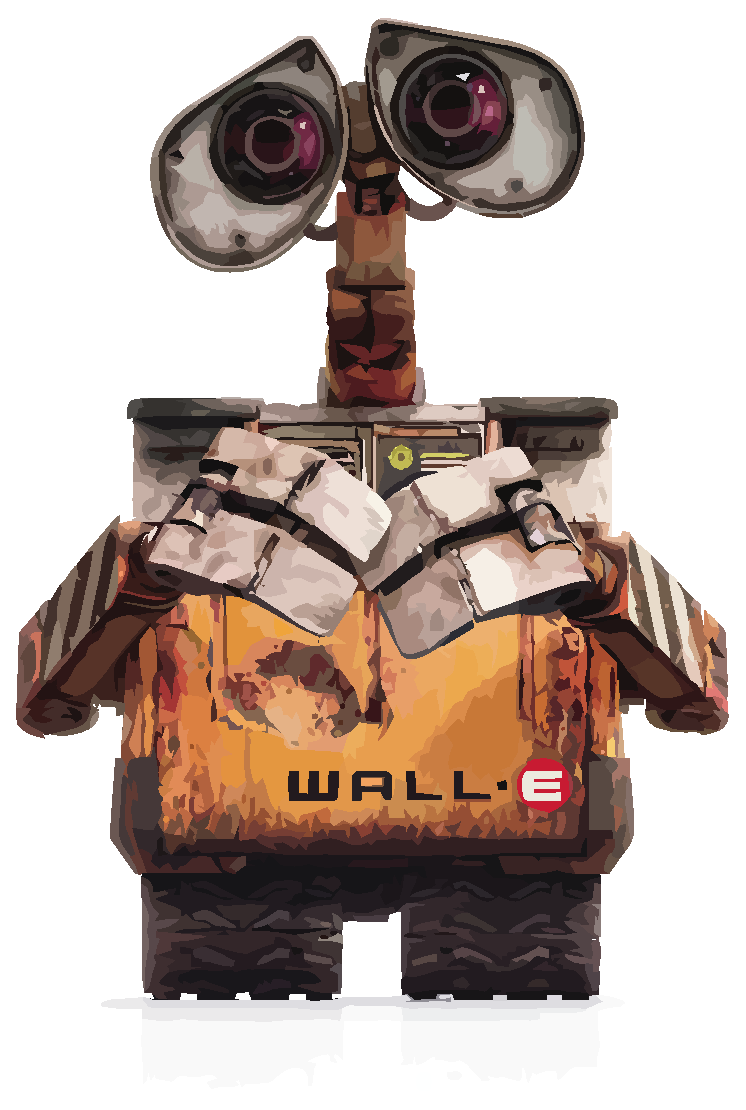
\includegraphics[width=\textwidth]{WallE}
    \caption{Wall-E}
    \label{fig:WallE}
  \end{subfigure}             
  \begin{subfigure}[b]{0.3\textwidth}
    
\includegraphics[width=\textwidth]{minion}
    \caption{Minions}
    \label{fig:Minnion}
  \end{subfigure}
  \caption{Best Animations}
  \label{fig:animations}
\end{figure}


\end{landscape}

%\chapter{My third chapter}

% **************************** Define Graphics Path **************************
\ifpdf
    \graphicspath{{Chapter3/Figs/Raster/}{Chapter3/Figs/PDF/}{Chapter3/Figs/}}
\else
    \graphicspath{{Chapter3/Figs/Vector/}{Chapter3/Figs/}}
\fi

\section{First section of the third chapter}
And now I begin my third chapter here \dots

And now to cite some more people~\citet{Rea85,Ancey1996}

\subsection{First subsection in the first section}
\dots and some more 

\subsection{Second subsection in the first section}
\dots and some more \dots

\subsubsection{First subsub section in the second subsection}
\dots and some more in the first subsub section otherwise it all looks the same
doesn't it? well we can add some text to it \dots

\subsection{Third subsection in the first section}
\dots and some more \dots

\subsubsection{First subsub section in the third subsection}
\dots and some more in the first subsub section otherwise it all looks the same
doesn't it? well we can add some text to it and some more and some more and
some more and some more and some more and some more and some more \dots

\subsubsection{Second subsub section in the third subsection}
\dots and some more in the first subsub section otherwise it all looks the same
doesn't it? well we can add some text to it \dots

\section{Second section of the third chapter}
and here I write more \dots

\section{The layout of formal tables}
This section has been modified from ``Publication quality tables in \LaTeX*''
 by Simon Fear.

The layout of a table has been established over centuries of experience and 
should only be altered in extraordinary circumstances. 

When formatting a table, remember two simple guidelines at all times:

\begin{enumerate}
  \item Never, ever use vertical rules (lines).
  \item Never use double rules.
\end{enumerate}

These guidelines may seem extreme but I have
never found a good argument in favour of breaking them. For
example, if you feel that the information in the left half of
a table is so different from that on the right that it needs
to be separated by a vertical line, then you should use two
tables instead. Not everyone follows the second guideline:

There are three further guidelines worth mentioning here as they
are generally not known outside the circle of professional
typesetters and subeditors:

\begin{enumerate}\setcounter{enumi}{2}
  \item Put the units in the column heading (not in the body of
          the table).
  \item Always precede a decimal point by a digit; thus 0.1
      {\em not} just .1.
  \item Do not use `ditto' signs or any other such convention to
      repeat a previous value. In many circumstances a blank
      will serve just as well. If it won't, then repeat the value.
\end{enumerate}

A frequently seen mistake is to use `\textbackslash begin\{center\}' \dots `\textbackslash end\{center\}' inside a figure or table environment. This center environment can cause additional vertical space. If you want to avoid that just use `\textbackslash centering'


\begin{table}
\caption{A badly formatted table}
\centering
\label{table:bad_table}
\begin{tabular}{|l|c|c|c|c|}
\hline 
& \multicolumn{2}{c}{Species I} & \multicolumn{2}{c|}{Species II} \\ 
\hline
Dental measurement  & mean & SD  & mean & SD  \\ \hline 
\hline
I1MD & 6.23 & 0.91 & 5.2  & 0.7  \\
\hline 
I1LL & 7.48 & 0.56 & 8.7  & 0.71 \\
\hline 
I2MD & 3.99 & 0.63 & 4.22 & 0.54 \\
\hline 
I2LL & 6.81 & 0.02 & 6.66 & 0.01 \\
\hline 
CMD & 13.47 & 0.09 & 10.55 & 0.05 \\
\hline 
CBL & 11.88 & 0.05 & 13.11 & 0.04\\ 
\hline 
\end{tabular}
\end{table}

\begin{table}
\caption{A nice looking table}
\centering
\label{table:nice_table}
\begin{tabular}{l c c c c}
\hline 
\multirow{2}{*}{Dental measurement} & \multicolumn{2}{c}{Species I} & \multicolumn{2}{c}{Species II} \\ 
\cline{2-5}
  & mean & SD  & mean & SD  \\ 
\hline
I1MD & 6.23 & 0.91 & 5.2  & 0.7  \\

I1LL & 7.48 & 0.56 & 8.7  & 0.71 \\

I2MD & 3.99 & 0.63 & 4.22 & 0.54 \\

I2LL & 6.81 & 0.02 & 6.66 & 0.01 \\

CMD & 13.47 & 0.09 & 10.55 & 0.05 \\

CBL & 11.88 & 0.05 & 13.11 & 0.04\\ 
\hline 
\end{tabular}
\end{table}


\begin{table}
\caption{Even better looking table using booktabs}
\centering
\label{table:good_table}
\begin{tabular}{l c c c c}
\toprule
\multirow{2}{*}{Dental measurement} & \multicolumn{2}{c}{Species I} & \multicolumn{2}{c}{Species II} \\ 
\cmidrule{2-5}
  & mean & SD  & mean & SD  \\ 
\midrule
I1MD & 6.23 & 0.91 & 5.2  & 0.7  \\

I1LL & 7.48 & 0.56 & 8.7  & 0.71 \\

I2MD & 3.99 & 0.63 & 4.22 & 0.54 \\

I2LL & 6.81 & 0.02 & 6.66 & 0.01 \\

CMD & 13.47 & 0.09 & 10.55 & 0.05 \\

CBL & 11.88 & 0.05 & 13.11 & 0.04\\ 
\bottomrule
\end{tabular}
\end{table}

%\include{Chapter4/chapter4}
%\include{Chapter5/chapter5}
%\include{Chapter6/chapter6}
%\include{Chapter7/chapter7}



% ********************************** Back Matter *******************************
% Backmatter should be commented out, if you are using appendices after References
%\backmatter

% ********************************** Bibliography ******************************
\begin{spacing}{0.9}

% To use the conventional natbib style referencing
% Bibliography style previews: http://nodonn.tipido.net/bibstyle.php
% Reference styles: http://sites.stat.psu.edu/~surajit/present/bib.htm

%\bibliographystyle{apalike}
\bibliographystyle{unsrt} % Use for unsorted references  
%\bibliographystyle{plainnat} % use this to have URLs listed in References
%\cleardoublepage
%\bibliography{References/references} % Path to your References.bib file


% If you would like to use BibLaTeX for your references, pass `custombib' as
% an option in the document class. The location of 'reference.bib' should be
% specified in the preamble.tex file in the custombib section.
% Comment out the lines related to natbib above and uncomment the following line.

%\printbibliography[heading=bibintoc, title={References}]


\end{spacing}

\end{document}


% ********************************** Appendices ********************************



\begin{appendices} % Using appendices environment for more functunality

% ******************************* Thesis Appendix A ****************************
\chapter{How to install \LaTeX} 

\section*{Windows OS}

\subsection*{TeXLive package - full version}
\begin{enumerate}
\item	Download the TeXLive ISO (2.2GB) from\\
\href{https://www.tug.org/texlive/}{https://www.tug.org/texlive/}
\item	Download WinCDEmu (if you don't have a virtual drive) from \\
\href{http://wincdemu.sysprogs.org/download/}
{http://wincdemu.sysprogs.org/download/}
\item	To install Windows CD Emulator follow the instructions at\\
\href{http://wincdemu.sysprogs.org/tutorials/install/}
{http://wincdemu.sysprogs.org/tutorials/install/}
\item	Right click the iso and mount it using the WinCDEmu as shown in \\
\href{http://wincdemu.sysprogs.org/tutorials/mount/}{
http://wincdemu.sysprogs.org/tutorials/mount/}
\item	Open your virtual drive and run setup.pl
\end{enumerate}

or

\subsection*{Basic MikTeX - \TeX~ distribution}
\begin{enumerate}
\item	Download Basic-MiK\TeX (32bit or 64bit) from\\
\href{http://miktex.org/download}{http://miktex.org/download}
\item	Run the installer 
\item	To add a new package go to Start >> All Programs >> MikTex >> Maintenance (Admin) and choose Package Manager
\item	Select or search for packages to install
\end{enumerate}

\subsection*{TexStudio - \TeX~ editor}
\begin{enumerate}
\item	Download TexStudio from\\
\href{http://texstudio.sourceforge.net/\#downloads}
{http://texstudio.sourceforge.net/\#downloads} 
\item	Run the installer
\end{enumerate}

\section*{Mac OS X}
\subsection*{MacTeX - \TeX~ distribution}
\begin{enumerate}
\item	Download the file from\\
\href{https://www.tug.org/mactex/}{https://www.tug.org/mactex/}
\item	Extract and double click to run the installer. It does the entire configuration, sit back and relax.
\end{enumerate}

\subsection*{TexStudio - \TeX~ editor}
\begin{enumerate}
\item	Download TexStudio from\\
\href{http://texstudio.sourceforge.net/\#downloads}
{http://texstudio.sourceforge.net/\#downloads} 
\item	Extract and Start
\end{enumerate}


\section*{Unix/Linux}
\subsection*{TeXLive - \TeX~ distribution}
\subsubsection*{Getting the distribution:}
\begin{enumerate}
\item	TexLive can be downloaded from\\
\href{http://www.tug.org/texlive/acquire-netinstall.html}
{http://www.tug.org/texlive/acquire-netinstall.html}.
\item	TexLive is provided by most operating system you can use (rpm,apt-get or yum) to get TexLive distributions
\end{enumerate}

\subsubsection*{Installation}
\begin{enumerate}
\item	Mount the ISO file in the mnt directory
\begin{verbatim}
mount -t iso9660 -o ro,loop,noauto /your/texlive####.iso /mnt
\end{verbatim}

\item	Install wget on your OS (use rpm, apt-get or yum install)
\item	Run the installer script install-tl.
\begin{verbatim}
	cd /your/download/directory
	./install-tl
\end{verbatim}
\item	Enter command `i' for installation

\item	Post-Installation configuration:\\
\href{http://www.tug.org/texlive/doc/texlive-en/texlive-en.html\#x1-320003.4.1}
{http://www.tug.org/texlive/doc/texlive-en/texlive-en.html\#x1-320003.4.1} 
\item	Set the path for the directory of TexLive binaries in your .bashrc file
\end{enumerate}

\subsubsection*{For 32bit OS}
For Bourne-compatible shells such as bash, and using Intel x86 GNU/Linux and a default directory setup as an example, the file to edit might be \begin{verbatim}
edit $~/.bashrc file and add following lines
PATH=/usr/local/texlive/2011/bin/i386-linux:$PATH; 
export PATH 
MANPATH=/usr/local/texlive/2011/texmf/doc/man:$MANPATH;
export MANPATH 
INFOPATH=/usr/local/texlive/2011/texmf/doc/info:$INFOPATH;
export INFOPATH
\end{verbatim}
\subsubsection*{For 64bit OS}
\begin{verbatim}
edit $~/.bashrc file and add following lines
PATH=/usr/local/texlive/2011/bin/x86_64-linux:$PATH;
export PATH 
MANPATH=/usr/local/texlive/2011/texmf/doc/man:$MANPATH;
export MANPATH 
INFOPATH=/usr/local/texlive/2011/texmf/doc/info:$INFOPATH;
export INFOPATH

\end{verbatim}



%\subsection{Installing directly using Linux packages} 
\subsubsection*{Fedora/RedHat/CentOS:}
\begin{verbatim} 
sudo yum install texlive 
sudo yum install psutils 
\end{verbatim}


\subsubsection*{SUSE:}
\begin{verbatim}
sudo zypper install texlive
\end{verbatim}


\subsubsection*{Debian/Ubuntu:}
\begin{verbatim} 
sudo apt-get install texlive texlive-latex-extra 
sudo apt-get install psutils
\end{verbatim}

% ******************************* Thesis Appendix B ********************************

\chapter{Installing the CUED class file}

\LaTeX.cls files can be accessed system-wide when they are placed in the
<texmf>/tex/latex directory, where <texmf> is the root directory of the user’s \TeX installation. On systems that have a local texmf tree (<texmflocal>), which
may be named ``texmf-local'' or ``localtexmf'', it may be advisable to install packages in <texmflocal>, rather than <texmf> as the contents of the former, unlike that of the latter, are preserved after the \LaTeX system is reinstalled and/or upgraded.

It is recommended that the user create a subdirectory <texmf>/tex/latex/CUED for all CUED related \LaTeX class and package files. On some \LaTeX systems, the directory look-up tables will need to be refreshed after making additions or deletions to the system files. For \TeX Live systems this is accomplished via executing ``texhash'' as root. MIK\TeX users can run ``initexmf -u'' to accomplish the same thing.

Users not willing or able to install the files system-wide can install them in their personal directories, but will then have to provide the path (full or relative) in addition to the filename when referring to them in \LaTeX.



\end{appendices}

% *************************************** Index ********************************
\printthesisindex % If index is present

\end{document}
